\documentclass[11pt]{article}

% --- Paquets de base ---
\usepackage[utf8]{inputenc}
\usepackage[T1]{fontenc}
\usepackage[french]{babel}
\usepackage{amsmath, amsfonts, amssymb}
\usepackage{geometry}
\geometry{a4paper, margin=1in}

% --- Mise en page et Style ---
\usepackage{titlesec}
\usepackage{enumitem}
\usepackage{booktabs}
\usepackage{longtable}
\usepackage{xcolor}
\usepackage{tcolorbox}
\usepackage{tikz}
\usepackage{hyperref}
\usepackage{caption}
\usepackage{graphicx}
\usetikzlibrary{shapes.geometric, arrows.meta, positioning, calc}

% --- Macros Mathématiques ---
\newcommand{\E}{\mathbb{E}}
\newcommand{\Prob}{\mathbb{P}}
\newcommand{\R}{\mathbb{R}}
\newcommand{\N}{\mathbb{N}}
\newcommand{\Var}{\mathrm{Var}}
\newcommand{\Cov}{\mathrm{Cov}}
\newcommand{\calN}{\mathcal{N}}
\newcommand{\calF}{\mathcal{F}}
\newcommand{\ind}{\mathbf{1}}

% --- Boîtes de définition ---
\tcbuselibrary{skins, breakable}
\newtcolorbox{definitionbox}[1][]{
  colback=gray!8, colframe=black!60,
  fonttitle=\bfseries, title=#1,
  sharp corners, boxrule=0.6pt, breakable
}
\newtcolorbox{noveltybox}[1][]{
  colback=blue!4, colframe=blue!50,
  fonttitle=\bfseries, title=#1,
  sharp corners, boxrule=0.8pt, breakable
}
\newtcolorbox{resourcebox}[1][]{
  colback=green!4, colframe=green!50,
  fonttitle=\bfseries, title=#1,
  sharp corners, boxrule=0.6pt, breakable
}
\newtcolorbox{resultbox}[1][]{
  colback=orange!6, colframe=orange!60!black,
  fonttitle=\bfseries, title=#1,
  sharp corners, boxrule=0.8pt, breakable
}
\newtcolorbox{diagnosticbox}[1][]{
  colback=red!4, colframe=red!50,
  fonttitle=\bfseries, title=#1,
  sharp corners, boxrule=0.8pt, breakable
}

% --- Configuration des Titres ---
\titleformat{\section}
  {\Large\bfseries\color{black}}{\thesection}{1em}{}[\titlerule]
\titleformat{\subsection}
  {\large\bfseries\color{black}}{\thesubsection}{1em}{}
\titleformat{\subsubsection}
  {\bfseries\color{black}}{\thesubsubsection}{1em}{}

% --- Paramètres de paragraphe ---
\setlength{\parskip}{0.5em}
\setlength{\parindent}{0pt}

\title{Interprétabilité automatique de mails clients par Sparse Autoencoders\\
\large Application à la correspondance client d'EDF}
\author{Grégoire Pelletier}
\date{}

% =============================================================================
\begin{document}

% ─────────────────────────────────────────────────────────────────────────────
% PAGE DE GARDE
% ─────────────────────────────────────────────────────────────────────────────
\begin{titlepage}
\centering
\vspace*{1cm}
{\large Université Paris-Saclay --- Faculté des Sciences d'Orsay\par}
{\large Master 2 Mathématiques et Intelligence Artificielle\par}
\vspace{2cm}
{\Huge\bfseries Rapport de stage\par}
\vspace{0.5cm}
{\LARGE Interprétabilité automatique de mails clients par\\ Sparse Autoencoders\par}
\vspace{0.3cm}
{\Large\itshape Application à l'analyse interprétable de la\\ correspondance client d'EDF\par}
\vspace{0.6cm}
{\normalsize\itshape Version pour relecture EDF --- avant remise universitaire\par}
\vspace{1.9cm}

\begin{tabular}{ll}
\textbf{Auteur} & Grégoire Pelletier \\[0.3em]
\textbf{Entreprise d'accueil} & EDF R\&D --- Département SEQUOIA, groupe SOAD \\[0.3em]
\textbf{Lieu} & EDF Lab Paris-Saclay, 7 boulevard Gaspard Monge, 91120 Palaiseau \\[0.3em]
\textbf{Maître de stage} & Philippe Suignard (département SEQUOIA) \\[0.3em]
\textbf{Durée du stage} & 6 mois --- mars 2026 à septembre 2026 \\[0.3em]
\textbf{Confidentialité} & Diffusion restreinte --- document destiné à la relecture EDF \\[0.3em]
\end{tabular}

\vfill
{\large \today\par}
\end{titlepage}

\newpage
\section*{Remerciements}
\addcontentsline{toc}{section}{Remerciements}

Je tiens à remercier Philippe Suignard, Claire Del Gatto et l'ensemble de
l'équipe du groupe Statistiques et Outils d'Aide à la Décision (SOAD) du
département SEQUOIA d'EDF R\&D pour leur accueil, leur disponibilité, la
liberté qui m'a été laissée d'explorer mes propres pistes et hypothèses tout
au long de ce stage, et les échanges réguliers et enrichissants sur les cas
d'usage industriels d'EDF qui ont accompagné ce travail. Je remercie
également EDF R\&D pour l'accès aux clusters de calcul GPU (H100, H100-bis,
A100) mis à ma disposition : une ressource sans laquelle la campagne
expérimentale de ce stage n'aurait tout simplement pas été possible. Je remercie chaleureusement les responsables et l'équipe pédagogique du Master 2 Mathématiques et Intelligence Artificielle de l'Université Paris-Saclay pour la qualité de la formation et leur suivi tout au long de cette année.

\newpage
\section*{Résumé}
\addcontentsline{toc}{section}{Résumé}

Ce stage étudie l'interprétabilité automatique de représentations textuelles denses par
Sparse Autoencoders (SAE), avec comme cas d'usage l'analyse de la correspondance
client d'EDF. L'objectif est double : construire une représentation parcimonieuse
permettant de relier les dimensions latentes à des concepts lisibles, et déterminer
dans quelle mesure cette représentation conserve une utilité opérationnelle pour des
tâches avales.

Deux pipelines indépendants ont été développés. Le premier étend un SAE GemmaScope
préentraîné par une extension à cœur gelé, entraînée sur le résidu non reconstruit du
cœur. Le second entraîne un SAE directement sur des embeddings de phrase multilingues
(F2LLM-v2 et bge-m3). L'architecture principale constitue une réplication indépendante
et une adaptation au domaine de l'idée de SAE Boost, sur des embeddings issus de mails
français plutôt que sur les activations étudiées dans les travaux d'origine.

Le travail expérimental met surtout en évidence quatre enseignements. Premièrement,
la validité de l'architecture ne peut pas être déduite du seul taux d'auto-interprétation :
le gain de variance expliquée de l'extension est fortement supérieur à celui de
décodeurs figés aléatoires, et une mesure complémentaire de fidélité causale par
cross-entropy confirme cette supériorité. Deuxièmement, le score d'interprétabilité est
très sensible au protocole expérimental : la sélection des features par magnitude et
la sélection stratifiée ne sondent pas la même population de features, tandis que le
choix du juge et la construction du négatif peuvent modifier substantiellement la
mesure. Le protocole final retenu combine sélection stratifiée, juge indépendant et
négatif corrigé. Troisièmement, l'effet d'échelle du modèle, initialement considéré
comme central, ne se réplique pas sous ce protocole : sur 1B, 4B, 12B et 27B, aucune
tendance monotone n'est détectée. Enfin, les expériences de stabilité montrent que les
features individuelles et certains regroupements doivent être interprétés avec
prudence, tandis que les codes SAE restent compétitifs avec une baseline TF-IDF sur
cinq tâches de détection d'intention.

Le résultat principal du stage est donc moins l'identification d'un optimum unique que
la construction d'une chaîne de validation qui distingue reconstruction, fidélité,
interprétabilité, robustesse et utilité applicative. Plusieurs pistes restent ouvertes,
notamment la réplication inter-seed de l'étude d'échelle, la validation du diffing sur
un corpus d'emails annoté et une comparaison plus large des backbones d'embedding.

\textbf{Mots-clés} : Sparse Autoencoders, interprétabilité mécaniste, GemmaScope,
explicabilité, embeddings, traitement automatique des mails, auto-interprétation par
juge LLM.

\newpage
\tableofcontents
\newpage
\listoffigures
\listoftables
\newpage

\section*{Glossaire}
\addcontentsline{toc}{section}{Glossaire}
\begin{description}[leftmargin=3.2cm, style=nextline]
  \item[SAE] Sparse Autoencoder (autoencodeur creux) : réseau qui reconstruit un
    vecteur d'entrée à partir d'une représentation intermédiaire parcimonieuse.
  \item[Feature] Une coordonnée du code latent produit par un SAE. Dans
    l'idéal, chaque feature s'active pour un unique concept sémantique
    identifiable (\emph{ex.} \og{}réclamation liée à la facturation\fg{}), et
    seulement pour lui --- c'est cette correspondance, quand elle est
    vérifiée, qui rend le modèle interprétable.
  \item[LLM] Large Language Model (grand modèle de langage).
  \item[GemmaScope] Famille de SAE préentraînés par Google DeepMind sur les
    activations des modèles Gemma/Gemma-2/Gemma-3 \cite{lieberum2024gemmascope}.
  \item[Neuronpedia] Plateforme externe hébergeant un catalogue de labels
    (générés par LLM, parfois validés humainement) déjà associés à chaque
    feature de nombreux SAE publiés, dont GemmaScope --- utilisée ici comme
    source de labels initiaux, complétée par le juge LLM local de ce stage.
  \item[L0] Pseudo-norme comptant le nombre de coordonnées non nulles d'un
    vecteur --- mesure la parcimonie effective d'un code SAE.
  \item[NMSE] Normalized Mean Squared Error --- erreur de reconstruction
    normalisée par la variance du signal d'origine.
  \item[FVE] Fraction de Variance Expliquée (parfois notée $R^2$).
  \item[$\Delta$CE] Augmentation de la perte d'entropie croisée (\emph{cross-entropy})
    du modèle lorsqu'on remplace l'activation réelle par sa reconstruction SAE
    --- mesure la fidélité \emph{fonctionnelle} de la reconstruction (son effet
    sur les prédictions du modèle), pas seulement sa fidélité géométrique.
  \item[BH / FDR] Correction de Benjamini-Hochberg pour comparaisons
    multiples --- contrôle le taux de faux positifs attendu (\emph{False
    Discovery Rate}) plutôt que le risque global d'au moins un faux positif.
  \item[MRL] Matryoshka Representation Learning --- apprentissage d'embeddings
    dont les préfixes de dimensions sont eux-mêmes des embeddings valides.
  \item[BM25] Fonction de pondération classique en recherche d'information,
    ici appliquée au vocabulaire latent d'un SAE (Latent Terms).
  \item[odd-one-out] Protocole d'auto-interprétation : un juge LLM doit
    identifier l'intrus parmi des extraits activant fortement une même feature.
  \item[McNemar] Test statistique apparié pour comparer deux proportions
    mesurées sur les mêmes unités d'observation sous deux conditions.
  \item[Cochran-Armitage] Test de tendance pour une variable binaire face à un
    facteur ordonné à plusieurs niveaux.
\end{description}

\newpage
% ─────────────────────────────────────────────────────────────────────────────
\section{Introduction et contexte}
% ─────────────────────────────────────────────────────────────────────────────

\subsection{Contexte industriel}

Ce stage s'est déroulé au sein d'EDF R\&D, dans le département SEQUOIA
(\textbf{S}ervices, \textbf{É}conomie, \textbf{Q}uestions h\textbf{U}maines,
\textbf{O}utils \textbf{I}nnovants et I\textbf{A}), qui éclaire le Groupe EDF
sur les sujets de transitions énergétique, numérique et sociétale du secteur et conçoit
les outils --- data analytics, IA, sciences humaines et sociales --- au
service de la connaissance client et de la relation client. Le stage a été
réalisé au sein du groupe de recherche SOAD (Statistiques et Outils d'Aide à
la Décision), équipe E7S, sur le site d'EDF Lab Paris-Saclay. La mission
initiale, formulée par l'offre de stage
(\emph{cf.}~annexe des sources), porte sur l'explicabilité des
\textbf{embeddings de texte} : des vecteurs denses obtenus par transformation
d'un document textuel, aujourd'hui massivement utilisés (classification,
recherche de documents similaires) mais dont la production reste, par
construction, une boîte noire. Les Sparse Autoencoders (SAE), apparus
récemment en interprétabilité mécaniste, sont identifiés par l'offre de stage
comme une piste prometteuse pour lever ce verrou.

Le cas d'usage retenu pour ancrer cette investigation méthodologique est
l'analyse de mails clients reçus par EDF : un volume important de
correspondance dont le traitement (priorisation, orientation vers le bon
service, détection des réclamations et des urgences) est aujourd'hui coûteux à
automatiser de façon à la fois efficace et interprétable --- un préalable
important dans un contexte réglementé où une décision automatisée doit
pouvoir être justifiée.

\subsection{Fondements théoriques : polysémanticité et superposition}

Les grands modèles de langage offrent une capacité de compréhension fine du
texte, mais leurs représentations internes restent largement opaques : une
même dimension de leur espace d'activation encode typiquement plusieurs
concepts sémantiques non corrélés, un phénomène appelé
\textbf{polysémanticité}. Il découle de l'hypothèse de \textbf{superposition}
\cite{elhage2022superposition} : contraints par une dimensionnalité fixe, les
réseaux de neurones compressent davantage de caractéristiques (\emph{features})
que de dimensions disponibles, en exploitant des directions quasi-orthogonales
de leur espace latent.

Cette question --- dans quelle mesure un LLM « comprend » réellement le texte
qu'il traite plutôt que d'en imiter la surface statistique --- est elle-même
débattue ; Beckmann \& Queloz \cite{beckmannqueloz2026} soutiennent que les avancées récentes de
l'interprétabilité mécanique rendent la position purement sceptique de moins
en moins tenable. Les Sparse Autoencoders proposent précisément de réapprendre
une représentation parcimonieuse et de plus haute dimension dans laquelle
chaque direction --- désormais appelée \textbf{feature} --- correspond, dans
l'idéal, à un concept isolé et nommable en langage naturel
\cite{bricken2023monosemanticity, cunningham2023sparse}. C'est cette
correspondance entre feature et concept que ce rapport cherche à mesurer,
via le taux d'\textbf{interprétabilité} : la proportion de features pour
lesquelles un concept partagé et identifiable est effectivement retrouvé.

\subsection{Objectifs du stage}

L'ambition du stage est de construire une plateforme d'analyse de
mails, les applications sont larges : l'indexation et la recherche par concept, le clustering
interprétable de documents, la détection d'urgence et d'intention, la
comparaison de corpus (\emph{diffing} : repérer automatiquement les features
dont l'activation moyenne diffère significativement entre deux sous-corpus,
\emph{ex.} les mails \og{}urgents\fg{} contre le reste, pour faire émerger ce
qui les distingue), la visualisation des concepts activés, le retrieval par
propriétés, et l'explication des décisions prises en aval de ces
représentations. Il est apparu que la communauté d'interprétabilité mécanistique était assez active, et il était logique de réutiliser au maximum
l'existant (SAELens, GemmaScope, la littérature sur l'interprétation
d'embeddings documentaires) plutôt que de réimplémenter, et de documenter
systématiquement les écarts avec ces références lorsqu'une réimplémentation
partielle s'avère nécessaire.

Une phase préliminaire de recherche bibliographique (état de l'art détaillé au
chapitre~\ref{sec:etat-art}) a permis de dresser un panorama des architectures
SAE et des modèles d'embeddings candidats, et de formuler plusieurs pistes de
contribution méthodologique (architecture hybride à cœur gelé, pipeline
micro/macro, dimensionnement des données). La suite du stage a consisté à
implémenter, tester empiriquement et, le cas échéant, corriger ces
hypothèses de travail sur des données réelles du domaine.

\begin{definitionbox}[Précision importante sur la nature du corpus]
Le corpus d'emails utilisé (\texttt{Mails.tsv}), désigné dans ce rapport par
commodité comme les mails \og{}originaux\fg{}, n'est \textbf{pas} de la
correspondance client authentique : il s'agit d'un jeu de données déjà
synthétique, produit par un travail antérieur du laboratoire EDF R\&D (non
réalisé pendant ce stage). Les variantes \emph{augmentées} sont, elles,
générées pendant ce stage (Gemma-3-12B-it) à partir de ces mails
\og{}originaux\fg{}. Aucune des deux couches du corpus n'est donc constituée
de données réelles au sens strict --- le terme \og{}original\fg{} désigne
uniquement leur statut de donnée d'entrée par rapport aux variantes qui en
dérivent, pas leur authenticité. Ce rappel s'applique à toute expérience de
ce rapport qui mobilise les mails \og{}originaux\fg{}, y compris celles du
chapitre~\ref{sec:resultats-utilite} portant sur la détection d'intention.
\end{definitionbox}

\subsection{Hypothèses de travail}

Les expériences ont été organisées autour de plusieurs questions qui permettent de
distinguer les propriétés de la représentation de celles du protocole d'évaluation ---
chacune est reprise, sous forme de question scientifique explicite, en tête du
chapitre de résultats qui y répond :
\begin{enumerate}
  \item \textbf{Domaine contre volume :} le manque de données dans le domaine cible
  explique-t-il l'échec initial, ou faut-il surtout augmenter le volume d'entraînement ?
  (chapitre~\ref{sec:resultats-representation})
  \item \textbf{Validité de la représentation :} l'extension à cœur gelé apprend-elle
  effectivement une information résiduelle utile, au-delà de ce qu'un dictionnaire
  aléatoire pourrait produire ? (chapitre~\ref{sec:resultats-representation})
  \item \textbf{Mesure de l'interprétabilité :} le score \emph{odd-one-out} est-il
  stable vis-à-vis de la population de features sélectionnée, du juge et de la
  construction du négatif ? (chapitre~\ref{sec:resultats-mesure})
  \item \textbf{Échelle et hyperparamètres :} les variations d'architecture, de layer,
  de parcimonie ou de taille du modèle produisent-elles des effets robustes une fois
  le protocole fixé ? (chapitre~\ref{sec:resultats-robustesse})
  \item \textbf{Stabilité :} les features et les structures de groupes observées sont-elles
  reproductibles entre graines et distinctes de structures obtenues aléatoirement ?
  (chapitre~\ref{sec:resultats-stabilite})
  \item \textbf{Utilité :} les représentations SAE apportent-elles une valeur mesurable
  sur des tâches avales indépendantes du score d'auto-interprétation ?
  (chapitre~\ref{sec:resultats-utilite})
\end{enumerate}

\subsection{Démarche et plan du rapport}

Le travail
s'est structuré autour d'un même fil directeur, répété à chaque étape :
diagnostiquer par ablation contrôlée plutôt que par intuition, puis valider
statistiquement avant de généraliser. Cette démarche a d'abord permis
d'identifier et de corriger un défaut de conception du corpus d'entraînement
de l'extension (\emph{cf.}~\S\ref{subsec:diagnostic-initial}), puis de la
réappliquer systématiquement à une large campagne d'ablations
d'hyperparamètres, jusqu'à la méthodologie statistique elle-même. Ce rapport suit une organisation thématique et non
chronologique : les choix d'architecture et les résultats sont présentés dans
leur forme aboutie, les étapes intermédiaires n'étant mentionnées que
lorsqu'elles éclairent directement une décision (\emph{cf.} notamment
\S\ref{subsec:diagnostic-initial} et \S\ref{subsec:sae-boost-litt}).

Le chapitre~\ref{sec:etat-art} positionne le projet par rapport à l'état de
l'art. Le chapitre~\ref{sec:contribution} décrit l'architecture et la
méthodologie mises en œuvre. Les résultats, cœur scientifique du rapport,
sont ensuite présentés en cinq chapitres organisés par question scientifique
plutôt que par ordre chronologique, chacun se refermant sur ce qu'il permet
d'affirmer :
\begin{itemize}
  \item le chapitre~\ref{sec:resultats-representation} établit si la
  représentation apprise par l'extension à cœur gelé est effectivement utile ;
  \item le chapitre~\ref{sec:resultats-mesure} examine ce que le protocole
  d'auto-interprétation mesure réellement ;
  \item le chapitre~\ref{sec:resultats-robustesse} teste la robustesse de ces
  conclusions aux choix d'échelle et d'hyperparamètres ;
  \item le chapitre~\ref{sec:resultats-stabilite} interroge la stabilité et
  l'identifiabilité des structures latentes ;
  \item le chapitre~\ref{sec:resultats-utilite} évalue l'utilité applicative
  de la représentation, indépendamment du score d'auto-interprétation.
\end{itemize}
Le chapitre~\ref{sec:discussion} discute enfin ce qui est établi, ce qui ne
l'est pas, les limites, les apports pour EDF et les perspectives, avant de
conclure.

\newpage
% ─────────────────────────────────────────────────────────────────────────────
\section{Méthodes, algorithmes et état de l'art}
\label{sec:etat-art}
% ─────────────────────────────────────────────────────────────────────────────

\subsection{Fondements théoriques de l'apprentissage de dictionnaires}

L'hypothèse de la représentation linéaire postule que les modèles de langage
représentent les concepts de haut niveau comme des directions linéaires dans
leur espace d'activation \cite{elhage2022superposition}. Soit une distribution
de données $D_x$ sur un espace d'entrée $\mathcal{X}$ (textes), et une
fonction d'activation interne $h : \mathcal{X} \rightarrow \mathbb{R}^{d_\text{model}}$
extraite d'un modèle. L'objectif de l'apprentissage de dictionnaire
parcimonieux est de trouver une matrice de décodage
$W_\text{dec} \in \mathbb{R}^{d_\text{model} \times d_\text{hidden}}$
($d_\text{hidden} \gg d_\text{model}$) et une fonction d'encodage
$f : \mathbb{R}^{d_\text{model}} \rightarrow \mathbb{R}^{d_\text{hidden}}$
produisant un vecteur d'activation latent $z = f(h(x))$ tel que la
reconstruction $\hat{h}(x) = W_\text{dec}\, z + b_\text{dec} \approx h(x)$ soit
fidèle, tandis que $z$ reste très parcimonieux ($\|z\|_0 \ll d_\text{hidden}$) :
chaque coordonnée $z_j$ est l'activation de la $j$-ième \textbf{feature}
(\emph{cf.}~glossaire), et sa nullité pour la quasi-totalité des entrées est
précisément ce qui rend chaque feature active potentiellement spécifique et
interprétable, plutôt que diffuse sur l'ensemble du corpus.

\begin{definitionbox}[Convention $W_\text{dec}$ --- nota bene]
Dans ce rapport, $W_\text{dec} \in \mathbb{R}^{d_\text{model} \times d_\text{hidden}}$
et chaque \textbf{colonne} $W_\text{dec}[:,j]$ est la direction de la $j$-ième
feature dans l'espace d'origine (convention Anthropic/Bricken 2023
\cite{bricken2023monosemanticity}). \textbf{SAELens \cite{bloom2024saelens}} (v6) stocke en revanche
\texttt{W\_dec} de forme \texttt{[d\_hidden, d\_model]} : la reconstruction est
alors $\hat{x} = \texttt{sae.W\_dec.T} \mathbin{@} z + \texttt{sae.b\_dec}$.
\end{definitionbox}

\subsection{Architectures des SAE}

\subsubsection{Standard SAE (ReLU, pénalité $L_1$)}
\[
  z = \text{ReLU}(W_\text{enc}(x - b_\text{pre}) + b_\text{enc}), \qquad
  \mathcal{L}_\text{Standard} = \|x - \hat{x}\|_2^2 + \lambda \|z\|_1
\]
Le gradient $\lambda\,\text{sgn}(z)$ pousse continûment chaque activation
active vers zéro, quelle que soit son amplitude réelle : $z$ sous-estime donc
systématiquement l'intensité du signal qu'il devrait porter, un biais dit de
\textbf{rétrécissement} (\emph{shrinkage}). Ce même gradient, en poussant
aussi les poids d'entrée vers zéro dès qu'une feature devient rarement
active, rend le Standard SAE particulièrement vulnérable aux latents morts
\cite{cunningham2023sparse}.

\subsubsection{Le problème des latents morts}

Un latent $j$ est dit \emph{mort} si son activation reste nulle sur un
horizon de batches consécutifs. Pour un Standard SAE, le gradient de la
pénalité $L_1$ pousse monotoniquement les poids vers zéro dès que la
pré-activation devient négative sur tout le batch, ce qui sature
irréversiblement la ReLU. Le diagnostic empirique se fait via
$\rho_\text{dead} = \frac{1}{d_\text{hidden}} \sum_j \ind[\max_x z_j(x) = 0]$ ;
un $\rho_\text{dead} > 5\%$ signale une compression excessive. Chaque
architecture propose son propre mécanisme anti-mort (séparation porte/magnitude
pour Gated, perte AuxK pour Top-K/BatchTopK, \emph{pre-act loss} et
initialisation de seuil pour JumpReLU) --- \emph{cf.}~état de l'art complet en
annexe des sources bibliographiques du stage.

\subsubsection{Gated SAE}
Sépare la décision d'activation (\emph{gate}) de sa magnitude
\cite{rajamanoharan2024gated} :
\[
  z = \ind(\pi_\text{gate}(x) > 0) \odot \text{ReLU}(\pi_\text{mag}(x)), \qquad
  \mathcal{L}_\text{Gated} = \|x - \hat{x}\|_2^2 + \lambda \|\text{ReLU}(\pi_\text{gate}(x))\|_1
\]
La pénalité $L_1$ ne porte que sur la porte : les magnitudes actives ne
subissent aucun rétrécissement.

\subsubsection{Top-K et BatchTopK}
Le Top-K contraint exactement $k$ latents actifs par exemple. Le
\textbf{BatchTopK} \cite{gao2024topk, bussmann2025batchtopk}, désormais
recommandé par SAELens comme architecture de référence, relaxe cette
contrainte à l'échelle du batch, avec une perte auxiliaire AuxK pour éviter
les latents morts :
\[
  \mathcal{L}_\text{BatchTopK} = \|x - \hat{x}\|_2^2 + \alpha\,\mathcal{L}_\text{AuxK}(e), \qquad
  \mathcal{L}_\text{AuxK}(e) = \bigl\|e - W_\text{dec}[:,\mathcal{S}]\,\text{TopK}(\pi_{\mathcal{D}_\text{dead}}, k_\text{aux})\bigr\|_2^2
\]

\subsubsection{JumpReLU}
Restaure une parcimonie adaptative sans pénalité $L_1$
\cite{rajamanoharan2024jumprelu} :
\[
  z_i = \pi_i(x) \cdot H(\pi_i(x) - \theta_i)
\]
où $\theta$ est un vecteur de seuils appris et $H$ la fonction de Heaviside.
La discontinuité rend le gradient nul presque partout ; les auteurs
utilisent un estimateur passe-droit (STE) avec approximation par noyau (KDE)
pour mettre à jour $\theta$.

\subsubsection{Matryoshka SAE}
Segmente le dictionnaire en sous-groupes emboîtés
$M = \{m_1 < m_2 < \dots < d_\text{hidden}\}$ et somme les erreurs de
reconstruction à chaque palier \cite{bussmann2025matryoshka} :
\[
  \mathcal{L}_\text{Matryoshka} = \sum_{m \in M} \omega_m \bigl\|x - (W_{\text{dec},\,0:m}\,z_{0:m} + b_\text{dec})\bigr\|_2^2
\]
Cette contrainte force les premières dimensions à encoder l'information la
plus saillante, avec une granularité adaptative à la clé (troncature sans
réentraînement).

\begin{table}[h!]
\centering
\caption{Comparaison analytique des architectures SAE}
\label{tab:sae-archs}
\vspace{0.5em}\small
\begin{tabular}{@{}lllll@{}}
\toprule
\textbf{Architecture} & \textbf{Mécanisme} & \textbf{Pénalité}
  & \textbf{Shrinkage} & \textbf{Statut} \\ \midrule
Standard  & $\text{ReLU}(\pi)$                          & $\lambda\|z\|_1$          & Non  & Baseline \\
Gated     & $\ind(\pi_g>0) \odot \text{ReLU}(\pi_m)$   & $\lambda\|\text{ReLU}(\pi_g)\|_1$ & Oui & Déprécié\\
Top-K     & Troncature $k$ max                          & AuxK                      & Oui  & Déprécié \\
BatchTopK & Troncature $n{\times}k$ max (batch)         & AuxK                      & Oui  & \textbf{Utilisé} \\
JumpReLU  & $\pi \cdot H(\pi - \theta)$                 & $\lambda\|z\|_0$ (STE)    & Oui  & Cœur préentraîné \\
Matryoshka & BatchTopK + nesting                        & $\sum_{m\in M}\|\cdot\|^2$ & Varie & Non implémenté \\ \bottomrule
\end{tabular}
\end{table}

\subsection{Choix du backbone d'embedding du second pipeline}

Le second pipeline (embeddings de phrase, indépendant de GemmaScope) s'appuie
sur \textbf{bge-m3} et la famille \textbf{F2LLM-v2} (80--330M paramètres),
retenus pour leur légèreté et, pour F2LLM-v2, leur support natif du
\textbf{Matryoshka Representation Learning} (MRL) \cite{kusupati2022mrl} : un
entraînement contrastif multi-résolution
($\mathcal{L}_{MRL} = \sum_{d \in \mathcal{D}} \omega_d \cdot
\mathcal{L}_\text{contrastive}(z_{1:d})$) qui rend chaque préfixe de
dimensions de l'embedding directement exploitable, sans réentraînement --- une
propriété testée empiriquement au chapitre~\ref{sec:resultats-utilite} et qui a
inspiré, dans la littérature SAE, l'architecture Matryoshka SAE (\emph{cf.}
Table~\ref{tab:sae-archs}). Le pipeline principal s'appuie quant à lui sur
GemmaScope, disponible \emph{prêt à l'emploi} avec un catalogue de labels
Neuronpedia déjà constitué --- un choix motivé par la disponibilité de cet
écosystème plutôt que par un score MTEB, discuté au
chapitre~\ref{sec:discussion}.

\subsection{Le SAE résiduel à cœur gelé : deux généalogies concurrentes}
\label{subsec:sae-boost-litt}

La piste architecturale retenue pour ce stage --- geler un SAE préentraîné et
entraîner une extension sur son résidu de reconstruction --- a été développée
en parallèle par ce projet et, dans la littérature publiée, par
\textbf{SAE Boost} \cite{koriagin2025saeboost} (Koriagin et al., juillet 2025) :

\begin{align*}
  e &= x - \hat{x}_\text{core} & \text{(résidu du SAE gelé)} \\
  z_\text{res} &= \text{BatchTopK}_{k_\text{res}}\bigl(\text{ReLU}(W_\text{enc}^{(\text{res})} x + b_\text{enc}^{(\text{res})})\bigr) \\
  \mathcal{L}_\text{Boost} &= \|e - \hat{e}\|_2^2 / \Var(e)
\end{align*}

Koriagin et al. rapportent des gains de +25\% à +59\% en variance expliquée
sur des domaines cibles (chimie, russe, débats ONU) pour moins de 1\% de
dégradation sur le domaine général.

\begin{definitionbox}[Pourquoi geler le cœur plutôt que réentraîner un SAE unique ?]
Si l'on réentraînait ou affinait un unique SAE partagé sur un mélange de texte
générique et de texte du domaine cible, les concepts des deux origines se
disputeraient le même budget fixe de features actives ($k$ dans BatchTopK).
Le SAE, pour minimiser son erreur de reconstruction, tend alors à
\textbf{réutiliser une même feature pour plusieurs concepts non liés} plutôt
que d'en dédier une par concept --- c'est cette \textbf{interférence de
routage} qui dégrade la monosémanticité, pour le domaine cible comme pour le
domaine général. Geler le cœur et n'entraîner qu'une extension sur le résidu
non reconstruit élimine ce partage \emph{par construction} : aucun budget de
sparsité n'est jamais mis en concurrence entre cœur et extension.
\end{definitionbox}

C'est l'architecture concrètement implémentée et
validée à l'échelle dans ce stage (\emph{cf.}~\S\ref{subsec:frozencore}) ---
et non une architecture Matryoshka pleinement hiérarchique et emboîtée, la
piste initialement envisagée en phase bibliographique préliminaire mais dont
la complexité d'entraînement et le besoin en données n'étaient pas justifiés
par les résultats obtenus (\emph{cf.}~chapitres~\ref{sec:resultats-representation}
à~\ref{sec:resultats-robustesse}).

\subsection{Sanity checks : les métriques proxy suffisent-elles ?}

Korznikov et al. \cite{korznikov2025sanitychecks} montrent qu'un SAE dont le
décodeur est figé à une initialisation aléatoire (jamais entraîné) atteint,
sur les métriques proxy usuelles (variance expliquée, AutoInterp
\cite{bills2023language}, sparse probing), des performances étonnamment
proches d'un SAE pleinement entraîné.
Ce résultat impose un critère de validation supplémentaire : toute
amélioration mesurée doit être évaluée \emph{relativement} à cette baseline
aléatoire gelée, et non uniquement en absolu. Ce protocole a été directement
reproduit dans ce stage (\emph{cf.}~\S\ref{subsec:sanity-check-resultats}).

\subsection{Interprétabilité au niveau documentaire}

L'application des SAE à des embeddings de documents entiers (plutôt qu'à des
activations token-level) constitue une extension récente de la littérature
\cite{jiang2024sae_embeddings, decodedense2025}. Le pipeline documentaire
distingue \textbf{interprétabilité globale} (que représente la feature $j$ sur
l'ensemble du corpus ? --- mesurée par juge LLM, protocole \emph{odd-one-out})
et \textbf{interprétabilité locale} (quelles features sont actives pour un
document donné ? --- mesurée par max-pooling documentaire des activations
token-level). Le protocole \emph{odd-one-out}
\cite{templeton2024scaling, karvonen2025saebench} présente au juge 9 extraits activant fortement une
même feature et 1 intrus aléatoire ; le juge doit identifier l'intrus, ce qui
ne peut réussir, par construction, que si les 9 extraits partagent un concept
identifiable.

\newpage
% ─────────────────────────────────────────────────────────────────────────────
\section{Contribution : architecture et méthodologie}
\label{sec:contribution}
% ─────────────────────────────────────────────────────────────────────────────

\subsection{Vue d'ensemble du système}

Le système implémente deux pipelines d'analyse interprétable de mails
clients EDF, partageant la même infrastructure de corpus, de stockage et
d'évaluation.

\begin{figure}[h!]
\centering
\begin{tikzpicture}[
  node distance=0.7cm and 0.8cm,
  box/.style={draw, rounded corners=2pt, minimum width=2.6cm, minimum height=0.8cm,
    align=center, font=\scriptsize, fill=gray!10},
  arrow/.style={-Stealth, thick}
]
  \node[box] (corpus) {Corpus principal\\Mails originaux +\\variantes augmentées};
  \node[box, below left=1.2cm and -0.3cm of corpus] (p1) {Pipeline 1\\Gemma-3-12B-it\\+ GemmaScope};
  \node[box, below right=1.2cm and -0.3cm of corpus] (p2) {Pipeline 2\\F2LLM-v2 / bge-m3\\+ PhraseLevelSAE};
  \node[box, below=0.9cm of p1] (ext) {Extension\\FrozenCoreResidualSAE\\(entraînée sur résidu)};
  \node[box, below=0.9cm of p2] (train) {SAE entraîné\\from-scratch};
  \node[box, below=0.9cm of ext] (pool1) {Max-pool\\documentaire};
  \node[box, below=0.9cm of train] (pool2) {Max-pool\\documentaire};
  \node[box, below=0.9cm of pool1] (lab1) {Labels : Neuronpedia\\+ juge LLM local};
  \node[box, below=0.9cm of pool2] (lab2) {Labels : juge LLM\\local (odd-one-out)};

  \draw[arrow] (corpus) -- (p1);
  \draw[arrow] (corpus) -- (p2);
  \draw[arrow] (p1) -- (ext);
  \draw[arrow] (p2) -- (train);
  \draw[arrow] (ext) -- (pool1);
  \draw[arrow] (train) -- (pool2);
  \draw[arrow] (pool1) -- (lab1);
  \draw[arrow] (pool2) -- (lab2);
\end{tikzpicture}
\caption{Architecture générale des deux pipelines d'analyse}
\label{fig:pipeline}
\end{figure}

\subsection{Architecture \texorpdfstring{$\textit{FrozenCoreResidualSAE}$}{FrozenCoreResidualSAE}}
\label{subsec:frozencore}

Pour aligner les embeddings d'origine (conçus majoritairement sur des corpus
anglophones) avec les spécificités sémantiques et techniques du corpus cible,
sans induire d'oubli catastrophique sur les capacités générales du SAE
préentraîné \cite{lieberum2024gemmascope}, le Pipeline~1 gèle le dictionnaire du cœur GemmaScope
($W_\text{dec}^\text{core}$) et instancie une extension de $D_\text{extra}$
features dédiées, entraînée exclusivement sur le résidu non reconstruit :
\[
  e = x - \hat{x}_\text{core} = x - \Bigl(b_\text{dec}^\text{core} +
  \sum_{j \in \mathcal{A}_\text{core}} z_j^\text{core}\, w_{\text{dec},j}^\text{core}\Bigr)
\]
\[
  z_\text{extra} = \text{BatchTopK}_{K_\text{extra}}\bigl(\text{ReLU}(W_\text{enc}^\text{extra} x + b_\text{enc}^\text{extra})\bigr), \qquad
  \hat{x} = \hat{x}_\text{core} + W_\text{dec}^\text{extra}\, z_\text{extra}
\]
Les poids $W_\text{dec}^\text{extra}$ sont initialisés par PCA sur un
sous-ensemble de calibration en français ; l'absence de biais additionnel
($b_\text{dec}^\text{extra}=0$) garantit que sur un flux hors-domaine
l'extension reste quasi-inactive, préservant la géométrie de base. Cette
architecture correspond exactement à celle décrite pour SAE Boost
(\S\ref{subsec:sae-boost-litt}) : les résultats de ce stage constituent donc,
\emph{de facto}, une réplication indépendante et une extension empirique de
cette architecture sur un nouveau domaine (embeddings emails clients français plutôt qu'activation de LLM) et à une
échelle de modèle non couverte par la publication d'origine
(1B/4B/12B~paramètres, \emph{cf.}~\S\ref{subsec:model-scale}).

\subsection{Métriques d'évaluation}

\subsubsection{Fidélité topologique locale : \texorpdfstring{$\rho_\text{SAE}$}{rho\_SAE}}
Pour vérifier que la projection SAE ne dénature pas la géométrie de l'espace
d'origine, on évalue la corrélation de rang de Spearman entre les matrices de
similarité cosinus calculées avant et après passage par le SAE, sur un
sous-ensemble de $N$ documents échantillonnés :
\[
  \rho_\text{SAE} = 1 - \frac{6\sum_{i=1}^n d_i^2}{n(n^2-1)}, \qquad
  d_i = \text{rang}(M_\text{raw}^{(i)}) - \text{rang}(M_\text{sae}^{(i)}), \qquad
  n = \binom{N}{2}
\]
Un $\rho_\text{SAE} \to 1$ valide empiriquement la conservation de la
topologie de l'espace de base.

\subsubsection{Sonde logistique (probing)}
Pour vérifier que la décomposition parcimonieuse préserve le pouvoir
discriminant, deux régressions logistiques multinomiales sont ajustées en
parallèle : $\text{Acc}_\text{raw}$ sur les embeddings denses d'origine
(borne supérieure oracle) et $\text{Acc}_\text{sae}$ sur les codes SAE. Le
différentiel $\Delta = \text{Acc}_\text{raw} - \text{Acc}_\text{sae}$ mesure
la perte d'information discriminante induite par la parcimonie. Au-delà de la
conservation de performance, cette sonde rend le modèle intrinsèquement
explicable : les coefficients $\beta_j^{(k)}$ les plus élevés isolent
directement les concepts sémantiques qui dictent la décision.

\subsubsection{Auto-interprétation par juge LLM}
Le taux d'interprétabilité rapporté dans tout ce rapport est mesuré par le
protocole \emph{odd-one-out} \cite{karvonen2025saebench} : pour chaque feature échantillonnée, un juge LLM
reçoit 9 documents activant fortement la feature et 1 document-contrôle
(activation quasi nulle), et doit désigner l'intrus. Un juge qui réussit
démontre l'existence d'un concept partagé identifiable ; l'échec ne prouve pas
nécessairement l'absence de concept (bruit du protocole,
\emph{cf.}~\S\ref{subsec:robustesse}). La campagne d'ablations
d'hyperparamètres du SAE (chapitre~\ref{sec:resultats-robustesse}) utilise le même modèle comme
extracteur et comme juge, par simplicité ; la valeur de référence retenue
pour ce rapport (65,7\%, \S\ref{subsec:protocole-final}) découple les deux
rôles, un juge de famille différente (Qwen3.8-27B) jugeant les features
extraites par Gemma-3-12B-it, pour écarter tout biais d'auto-préférence.

\subsection{Construction du corpus}

Le corpus principal combine les mails « originaux » (3\,480 documents,
\emph{cf.}~encadré \S\ref{sec:etat-art}) et leurs variantes augmentées
(39\,949 variantes acceptées sur 45\,240 générées, soit un taux de rejet de
qualité de 11,7\% --- \emph{cf.}~\S\ref{subsec:augmentation}), produites selon
13 axes de perturbation contrôlée (émotion, registre, orthographe, urgence).
Le split train/test est effectué au niveau du \textbf{mail d'origine} (et non
de la ligne) pour éviter qu'une variante augmentée d'un mail de test ne fuite
dans le train --- une variante et son mail source partagent un contenu
factuel quasi identique, ce qui biaiserait artificiellement les métriques de
classification en aval si elles se retrouvaient de part et d'autre du split.

\subsubsection{Garde-fou qualité de la génération augmentée}
\label{subsec:augmentation}
Chaque variante générée est soumise à un contrôle automatique (longueur
minimale, ratio de longueur par rapport au mail source dans $[0{,}4\,;\,2{,}5]$,
non-identité stricte, préservation des entités numériques du mail d'origine
sauf pour l'axe orthographe). 11,7\% des générations sont rejetées par ce
garde-fou, sans impact sur les résultats rapportés : les variantes rejetées
ne sont jamais chargées en aval de la génération.

\subsection{Protocole de validation et infrastructure}

L'ensemble des expériences a été exécuté sur un cluster SLURM à plusieurs
partitions GPU (A100/H100), sans accès réseau direct depuis les nœuds de
calcul --- toutes les dépendances (modèles, données) doivent être
prépositionnées sur disque avant soumission. Gemma-3 présente des activations
de norme très élevée (\emph{massive activations}) dans son flux résiduel ; une
précision fp16 (plage dynamique $\sim 65\,504$) provoque un dépassement
silencieux vers \texttt{inf}/\texttt{nan} sur ces valeurs, corrompant tout
entraînement en aval sans erreur explicite --- le projet utilise bf16 par
défaut partout, qui partage la plage d'exposant de fp32.

Le taux d'interprétabilité étant une proportion mesurée sur un échantillon de
$n=150$ features, chaque comparaison entre deux configurations est testée
statistiquement (test $z$ à deux proportions indépendantes par défaut ; test de
McNemar pour les comparaisons appariées sur les mêmes features ;
Cochran-Armitage pour les plans à niveaux ordonnés --- \emph{cf.}~la
discussion de puissance statistique \S\ref{subsec:ablations-finales}), avec
un seuil conventionnel de signification $|z| > 1{,}96$.

\newpage
% ─────────────────────────────────────────────────────────────────────────────
\section{Résultats : la représentation apprise est-elle utile ?}
\label{sec:resultats-representation}
% ─────────────────────────────────────────────────────────────────────────────

Avant de chercher à nommer les features par un juge LLM, encore faut-il établir
que l'extension à cœur gelé apprend effectivement une information résiduelle
réelle, plutôt que de reconstruire du bruit que l'auto-interprétation
habillerait \emph{a posteriori} d'un vocabulaire plausible. Ce chapitre répond
à cette question par quatre expériences complémentaires : le diagnostic du
corpus d'entraînement de l'extension, la comparaison à un décodeur figé
aléatoire, et deux métriques continues --- $\Delta$FVE et $\Delta$CE ---
délibérément choisies indépendantes du juge LLM et de la construction du
document négatif, dont la fragilité est établie au chapitre~\ref{sec:resultats-mesure}.

\subsection{Diagnostic et correction du problème initial}
\label{subsec:diagnostic-initial}

Le pipeline complet fonctionnait de bout en bout, mais le run disponible en
début de cette phase, jugé sur un échantillon initial d'une dizaine de
features seulement (corpus generic énergie/sport/support) --- bien trop
restreint pour être statistiquement exploitable, mais suffisant pour alerter
--- échouait le test \emph{odd-one-out} dans la grande majorité des cas.
L'inspection qualitative des exemples présentés au juge a révélé l'absence de
concept commun identifiable entre les 9 extraits
positifs d'une même feature (\emph{ex.} : rappel produit iPad, système
carcéral norvégien, recette de cuisine et agriculture canadienne présentés
ensemble). La lecture du code d'assemblage du corpus a montré la cause
racine : le réservoir de résidus servant à entraîner l'extension était
constitué \textbf{exclusivement} de texte générique (Wikipédia filtré par
mots-clés) --- les mails du domaine cible n'entraient jamais dans les données
d'entraînement de l'extension, seulement dans une visualisation post-hoc.

\begin{resultbox}[Correction et validation]
Une fois le corpus principal reconstruit (mails + variantes augmentées,
\S\ref{sec:contribution}) et le nombre de features jugées porté à 150 pour une
puissance statistique correcte, le taux d'interprétabilité passe à
\textbf{45,3\% (68/150)}, à volume de
tokens comparable. Faire varier ce volume d'un facteur 20 (100k à 2M tokens),
à domaine fixé, ne produit \textbf{aucun effet mesurable} (40,7\% / 45,3\% /
44,7\%, écarts non significatifs). \textbf{Le problème initial était donc un
défaut de domaine du corpus, pas un déficit de volume d'entraînement.}
\end{resultbox}

\subsection{Sanity check : le SAE bat-il un décodeur figé aléatoire ?}
\label{subsec:sanity-check-resultats}

Reproduisant le protocole de Korznikov et al.~\cite{korznikov2025sanitychecks}
(\S\ref{sec:etat-art}), un décodeur $W_\text{dec}^\text{extra}$ figé à une
initialisation aléatoire (jamais entraîné) atteint tout de même
\textbf{29,3\%} d'interprétabilité (44/150) --- nettement en dessous du SAE
pleinement entraîné (45,3\%, écart significatif, $z=2,86$) mais loin d'être
nul. Sur la métrique de classification (séparabilité des 14 classes d'axes
de perturbation), l'écart se resserre fortement (93,5\% entraîné contre
91,2\% figé) : \textbf{la classification en aval résiste beaucoup mieux à un
décodeur aléatoire que l'interprétation qualitative}, répliquant partiellement
le constat du papier sur des métriques proxy insuffisantes.

Cette mesure date de la sélection par magnitude et du juge auto-référent ---
rejouée sous méthodologie finale contre R0 (\S\ref{subsec:correction-methode}),
sous les deux schémas d'initialisation aléatoire de Korznikov et al.
(\emph{iso}, gaussienne isotrope ; \emph{cov}, gaussienne de covariance
réelle --- leur schéma \emph{principal}, empiriquement plus difficile à
battre). Dans les deux cas, un décodeur figé aléatoire laisse l'extension
massivement morte (98,9\% des 1024 directions sous \emph{iso}, 11 vivantes ;
97,0\% sous \emph{cov}, 31 vivantes --- contre 5,7\% pour R0), et le
$\Delta$FVE gagné par l'extension s'effondre en proportion : $+0{,}0001$
(\emph{iso}) et $+0{,}0086$ (\emph{cov}) contre $+0{,}1393$ pour R0 --- des
facteurs respectifs de ${\sim}1400$ et ${\sim}16$. \textbf{Même sous le
schéma le plus favorable au décodeur aléatoire, le SAE entraîné explique
${\sim}16\times$ plus de variance résiduelle supplémentaire.}

Sur le taux d'interprétabilité lui-même, la comparaison est plus fragile.
Une fois le biais de construction du négatif identifié et corrigé (audit
détaillé en \S\ref{subsec:audit-negatif}), les rares features vivantes du
décodeur aléatoire donnent \textbf{72,7\% ($n=11$) et 74,2\% ($n=31$)} ---
statistiquement indiscernables de R0 ($p=0{,}63$ et $p=0{,}34$), alors que
sous l'ancien protocole l'écart apparaissait significatif ($z=2{,}86$) :
\textbf{le signal distinguant décodeur entraîné et décodeur aléatoire sur le
seul taux d'interprétabilité ne survit pas à la correction du négatif}, à la
faible puissance disponible sur 11/31 features vivantes. C'est le
$\Delta$FVE, indépendant du bruit de jugement et de la construction du
négatif, qui reste le test de falsification net de ce sanity check --- pas
le taux d'interprétabilité, dont ce résultat confirme une fois de plus la
fragilité comme métrique isolée lorsqu'elle est utilisée seule.

\begin{figure}[h!]
\centering
\IfFileExists{figures/delta_fve_bars.png}{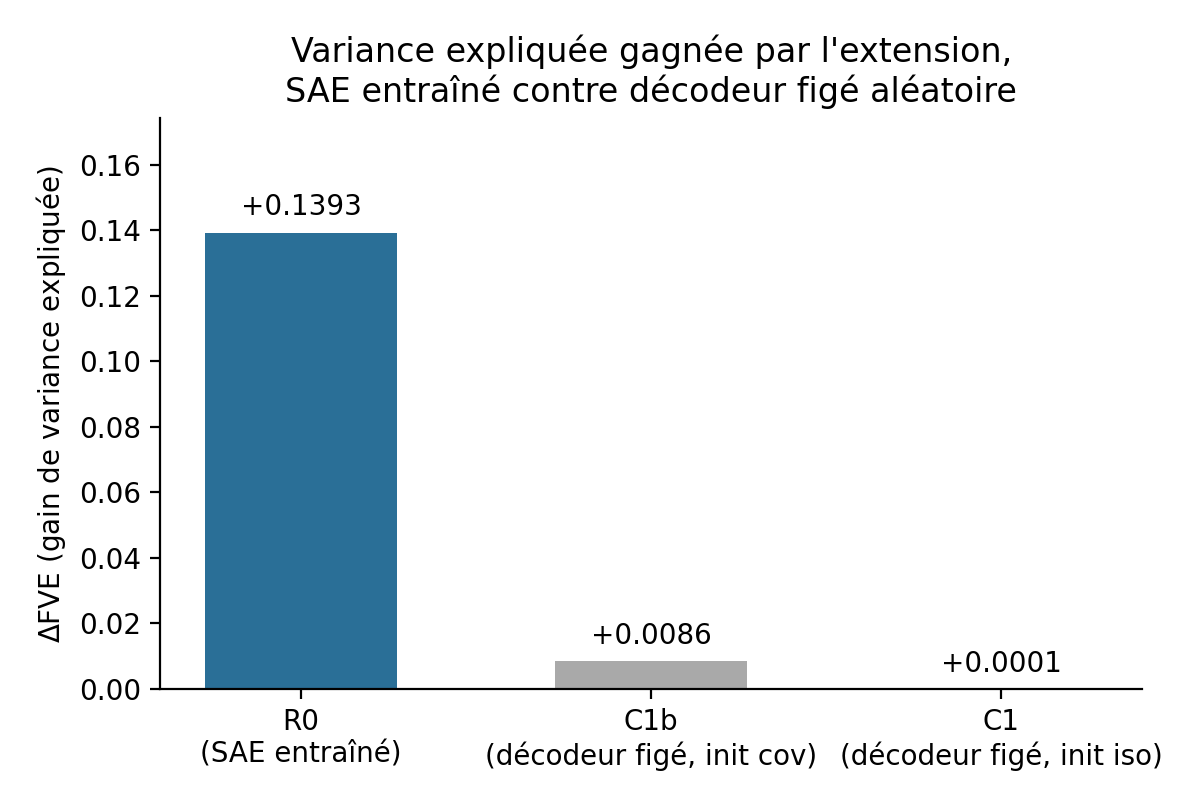
\includegraphics[width=0.7\textwidth]{figures/delta_fve_bars.png}}{\fbox{\parbox[c][4cm][c]{0.65\textwidth}{\centering Figure unavailable in standalone review export}}}
\caption{Variance expliquée gagnée par l'extension ($\Delta$FVE) : SAE
entraîné contre les deux sanity checks à décodeur figé aléatoire
(Korznikov et al.~\cite{korznikov2025sanitychecks}). Métrique continue,
indépendante du juge LLM et donc du biais de négatif
\S\ref{subsec:audit-negatif}.}
\label{fig:delta-fve}
\end{figure}

\subsection{Validation architecturale indépendante du juge : $\Delta$FVE et $\Delta$CE}
\label{subsec:delta-ce}

Le sanity check précédent conduit à distinguer deux questions : le taux
\emph{odd-one-out} permet-il de nommer les features, et l'extension apprend-elle
réellement à reconstruire une information absente du cœur préentraîné ? La seconde
question peut être étudiée sans juge LLM. En plus du $\Delta$FVE présenté ci-dessus,
une mesure de fidélité causale fondée sur la \textbf{cross-entropy patchée} compare la
dégradation produite lorsque la contribution de l'extension est supprimée à celle
observée avec un décodeur aléatoire.

Sur la configuration de référence, la suppression des composantes pertinentes de
l'extension réduit de façon nettement plus importante la performance mesurée par
cross-entropy que dans le témoin aléatoire : la dégradation causale apportée par
l'extension est réduite de \textbf{69\%} dans le témoin aléatoire par rapport au SAE
entraîné ($p=8\times10^{-12}$, test de Wilcoxon). Ce résultat est particulièrement
important parce qu'il est continu, indépendant du juge et indépendant de la
construction du document négatif.

\begin{resultbox}[Validation architecturale]
Les deux métriques convergent : le décodeur entraîné récupère une quantité substantielle
d'information résiduelle ($\Delta$FVE de $+0{,}1393$ sous R0, contre $+0{,}0001$ à
$+0{,}0086$ pour les témoins aléatoires) et cette information intervient causalement
dans la mesure de cross-entropy. Le taux d'auto-interprétation ne constitue donc pas
le seul argument en faveur de l'architecture à cœur gelé.
\end{resultbox}

\medskip
\noindent\textbf{Ce que ce chapitre établit.} L'extension à cœur gelé apprend
une information résiduelle mesurable et causalement utile. Ce résultat est
indépendant du juge LLM et de la construction du protocole d'auto-interprétation,
dont la fiabilité --- nettement plus incertaine --- est examinée au chapitre
suivant.

\newpage
% ─────────────────────────────────────────────────────────────────────────────
\section{Résultats : que mesure réellement le protocole d'interprétabilité ?}
\label{sec:resultats-mesure}
% ─────────────────────────────────────────────────────────────────────────────

Le chapitre précédent établit que l'extension apprend une information
résiduelle réelle. Reste à déterminer si le taux d'interprétabilité
\emph{odd-one-out}, utilisé pour nommer cette information, est lui-même une
mesure fiable. Ce chapitre traite le protocole de mesure comme une variable
expérimentale à part entière : la population de features évaluée, le choix
du juge, la construction du document négatif et la robustesse aux
perturbations de surface y sont chacun testés. C'est le résultat
méthodologique le plus transversal de ce stage, potentiellement transférable
à tout projet d'auto-interprétation par juge LLM.

\subsection{Sélection des features et choix du juge : deux variables expérimentales}
\label{subsec:correction-methode}

Le taux d'interprétabilité n'est pas une propriété observée directement : il dépend
d'une chaîne d'échantillonnage et de jugement. Deux dimensions de cette chaîne ont
été étudiées comme de véritables variables expérimentales.

La première est la \textbf{sélection des features}. Une sélection par magnitude
d'activation moyenne surreprésente les features les plus souvent et fortement
activées, alors qu'une sélection \textbf{stratifiée par fréquence} répartit
l'échantillon sur l'ensemble du dictionnaire. Cette comparaison répond à une question
méthodologique plus fine qu'un simple choix d'hyperparamètre : \emph{le score mesuré
caractérise-t-il le dictionnaire dans son ensemble, ou principalement ses directions
les plus denses et génériques ?} Formulée directement, la question qui structure ce
chapitre est : \textbf{le taux d'interprétabilité mesuré est-il une propriété du
dictionnaire de features dans son ensemble, ou seulement de la sous-population de
features que l'on choisit d'évaluer ?} C'est une question non triviale --- elle ne se
réduit pas à un choix d'hyperparamètre d'évaluation, puisqu'elle détermine si le
chiffre rapporté dans ce document caractérise le SAE ou le protocole qui l'a mesuré.

La seconde est le \textbf{choix du juge}. Le protocole oppose un juge de la même
famille que le modèle extracteur à un juge d'une famille indépendante (Qwen3.8-27B).
La comparaison permet de rechercher un éventuel biais d'auto-préférence sans confondre
ce facteur avec le choix de la population de features.

Les deux variables sont croisées sur une configuration commune
($K_\text{extra}=5$, $D_\text{extra}=1024$, 25M tokens, layer 31). Sous l'ancienne
construction du négatif, le passage de la sélection magnitude au schéma stratifié,
combiné au changement de juge, produisait un déplacement très important du taux
mesuré. Cette observation a motivé un audit indépendant de la construction du négatif
(\S\ref{subsec:audit-negatif}), qui a ensuite conduit à définir le protocole final
(\S\ref{subsec:protocole-final}). Le chiffre de référence retenu
n'est donc pas un résultat de la campagne historique, mais celui obtenu après
stabilisation de l'ensemble de la chaîne.

\subsection{Audit et correction du négatif odd-one-out}
\label{subsec:audit-negatif}

L'audit de la construction du document négatif illustre concrètement pourquoi
le protocole de mesure doit être traité comme une variable expérimentale à
part entière, plutôt que comme un détail d'implémentation. Il ne s'agit pas,
en soi, d'un résultat scientifique nouveau sur la représentation apprise :
c'est un \textbf{contrôle de validité du protocole}, qui conditionne
l'interprétation de toutes les mesures d'interprétabilité de ce rapport ---
et non la contribution centrale du stage.

\begin{resultbox}[Audit du négatif odd-one-out : un contrôle de validité du protocole]
Une inspection manuelle des exemples présentés au juge a révélé que le
document \og{}négatif\fg{} (censé ne pas partager le concept de la feature)
était, sur R0, plus court que chacun des 9 exemples positifs pour la
quasi-totalité des features --- souvent réduit à un mot de salutation ou de
ponctuation. \textbf{Cause racine} : le négatif est choisi parmi des
documents quasi-inactivants pour la feature (activation \textbf{exactement}
nulle, cas normal sous l'architecture parcimonieuse \emph{BatchTopK}) ; sur
un vecteur d'activation constant, l'argmax utilisé pour centrer le contexte
affiché renvoie systématiquement l'indice 0 (convention numpy sur les
ex-aequo) --- un artefact déterministe, pas une position de bruit distribuée,
qui ancre quasi tous les négatifs au tout début du document. \textbf{Un juge
peut alors résoudre la tâche par simple longueur/pauvreté de contexte, sans
lire le concept partagé par les 9 autres exemples}, pour l'écrasante majorité
des features de chaque run de ce stage --- un biais commun à toutes les
mesures d'interprétabilité antérieures à sa découverte. Le correctif retenu
tire une position aléatoire (graine déterministe, replay-stable) parmi les
débuts de mot à contexte suffisant lorsque le signal du candidat est nul, et
n'utilise l'argmax que lorsqu'il porte un signal réel.

\textbf{Rejugé sous ce correctif à $n=150$, R0 tombe de 84,7\% à 62,7\%} ---
un écart de 22 points, très supérieur au bruit d'échantillonnage attendu à
cette taille d'échantillon ($p=1{,}5\times10^{-5}$) : une fraction
substantielle du taux d'interprétabilité mesuré provenait de cet artefact,
pas d'une reconnaissance de concept par le juge. Rejugé à $n=300$ pour
resserrer la précision, R0 donne \textbf{65,7\% (197/300)}, IC95\%
$[60{,}1\%\,;\,70{,}8\%]$ --- statistiquement indiscernable de l'estimation à
$n=150$ ($p=0{,}53$) : c'est la valeur de référence retenue pour la suite de
ce rapport. \textbf{Ce biais ne réfute pas les résultats en $\Delta$FVE et
$\Delta$CE du chapitre~\ref{sec:resultats-representation}} (métriques
continues, indépendantes de la construction du négatif), mais il invalide la
valeur absolue de tout taux d'interprétabilité cité dans les versions
antérieures de ce document, y compris l'ancienne référence 84,7\% ---
\textbf{ainsi que la conclusion d'absence d'effet d'hyperparamètre et
d'effet d'échelle du modèle qui en avait été tirée} : rejugés à $n=300$
(\S\ref{subsec:ablations-finales}, \S\ref{subsec:model-scale}), la
quasi-totalité des hyperparamètres du SAE restent sans effet détectable ---
$K_\text{extra}$ fait exception --- et l'effet d'échelle du modèle,
initialement présenté comme un résultat central, ne réplique pas du tout
sous protocole intégralement corrigé.
\end{resultbox}

\subsection{Protocole final de référence}
\label{subsec:protocole-final}

\begin{resultbox}[Protocole de référence]
La configuration R0 retenue pour les comparaisons finales est : sélection stratifiée
par fréquence, juge indépendant Qwen3.8-27B, négatif corrigé, déduplication par mail
parent, $K_\text{extra}=5$, $D_\text{extra}=1024$, 25M tokens et layer 31. Elle donne
\textbf{65,7\% (197/300)}, IC95\% $[60{,}1\%\,;\,70{,}8\%]$.
Les valeurs historiques obtenues avant stabilisation du protocole sont conservées
comme comparaisons diagnostiques et non comme estimations finales.
\end{resultbox}

\subsection{Robustesse aux perturbations de surface (ordre, langue)}
\label{subsec:robustesse}

Deux tests évaluent la sensibilité du protocole \emph{odd-one-out} à des
perturbations de surface qui ne devraient, en principe, pas affecter le
jugement :

\begin{itemize}
  \item \textbf{Réordonnancement} : en répétant la question 5 fois par
    feature avec un ordre de présentation différent, seules 30,7\% des
    features obtiennent une décision unanime. Le taux agrégé bouge peu
    (single-shot 45,3\% contre vote majoritaire 48,7\%, test de McNemar
    $p=0,560$, non significatif) mais \textbf{31,3\% des features changent
    individuellement de statut} selon l'ordre de présentation.
  \item \textbf{Langue du juge} \cite{resck2025multilingual, multilingualconcepts2025} : traduire les exemples et le prompt en
    anglais ne change pas significativement le taux agrégé (français 46,9\%
    contre anglais 45,5\%, McNemar $p=0,894$), mais \textbf{38,6\% des
    features changent de statut} selon la langue --- un taux de bruit
    supérieur à celui du simple réordonnancement.
\end{itemize}

Ces deux résultats convergent vers la même conclusion : le protocole
\emph{odd-one-out} à décision unique est \textbf{génériquement bruyant} face
à toute perturbation de surface (ordre, langue), pas spécifiquement biaisé
dans une direction donnée. Un vote majoritaire sur plusieurs répétitions
devrait être préféré à une décision \emph{greedy} unique en usage de
production.

\medskip
\noindent\textbf{Ce que ce chapitre établit.} Le taux d'interprétabilité
\emph{odd-one-out} dépend fortement de la population de features évaluée, du
juge et de la construction du négatif ; une fois ces trois éléments audités
et corrigés, le protocole final (R0, 65,7\%) reste par ailleurs bruyant à
courte échelle (ordre, langue), mais offre une base de comparaison stable
pour les chapitres suivants.
\newpage
% ─────────────────────────────────────────────────────────────────────────────
\section{Résultats : les conclusions sont-elles robustes aux choix d'architecture et d'échelle ?}
\label{sec:resultats-robustesse}
% ─────────────────────────────────────────────────────────────────────────────

Le protocole de mesure étant désormais stabilisé (R0), ce chapitre teste si
les conclusions portées par ce protocole résistent aux choix d'échelle du
modèle et d'hyperparamètres du SAE, une fois la puissance statistique de
chaque comparaison explicitement prise en compte.

\subsection{L'échelle du modèle : un effet qui ne survit pas au protocole corrigé}
\label{subsec:model-scale}

Quatre échelles du modèle extracteur/juge sont testées sous une configuration
strictement commune (sélection stratifiée, juge Qwen3.8-27B, déduplication
par mail parent, $K_\text{extra}=5$, $D_\text{extra}=1024$, 25M tokens,
corpus mixte, négatif corrigé, $n=300$), chacune avec son propre GemmaScope
dédié et son propre \emph{layer} à \og{}~2/3 de profondeur\fg{}
\cite{formal2026splare} (1B : layer 13 ; 4B : layer 17 ; 12B : layer 31 ;
27B : layer 40) --- seul le \textbf{triplet} modèle/layer/SAE core varie
d'un point à l'autre, chaque layer étant la meilleure estimation
\og{}~2/3 profondeur\fg{} disponible pour son échelle : la taille du modèle
n'est donc pas isolée du layer dans ce sweep.

\begin{table}[h!]
\centering
\caption{Effet de l'échelle du modèle extracteur, méthodologie totalement homogène (stratifié, juge Qwen3.8-27B, négatif corrigé, $K_\text{extra}=5$, 25M tokens, $n=300$)}
\label{tab:model-scale}
\vspace{0.4em}\small
\begin{tabular}{@{}lcccc@{}}
\toprule
\textbf{Modèle} & \textbf{Layer} & \textbf{Taux interp.} & \textbf{IC95\% Wilson} & \textbf{$z$/$p$ vs R0} \\ \midrule
gemma-3-1b-it & 13 & 63,3\% (190/300) & [57,7\,;\,68,6] & $z=-0{,}60$, $p=0{,}55$ \\
gemma-3-4b-it & 17 & 54,7\% (164/300) & [49,0\,;\,60,2] & $z=-2{,}75$, $p=0{,}006$ \\
gemma-3-12b-it (référence, R0) & 31 & \textbf{65,7\% (197/300)} & [60,1\,;\,70,8] & --- \\
gemma-3-27b-it & 40 & 55,7\% (167/300) & [50,0\,;\,61,2] & $z=-2{,}51$, $p=0{,}012$ \\
\bottomrule
\end{tabular}
\end{table}

\begin{figure}[h!]
\centering
\IfFileExists{figures/model_scale_curve.png}{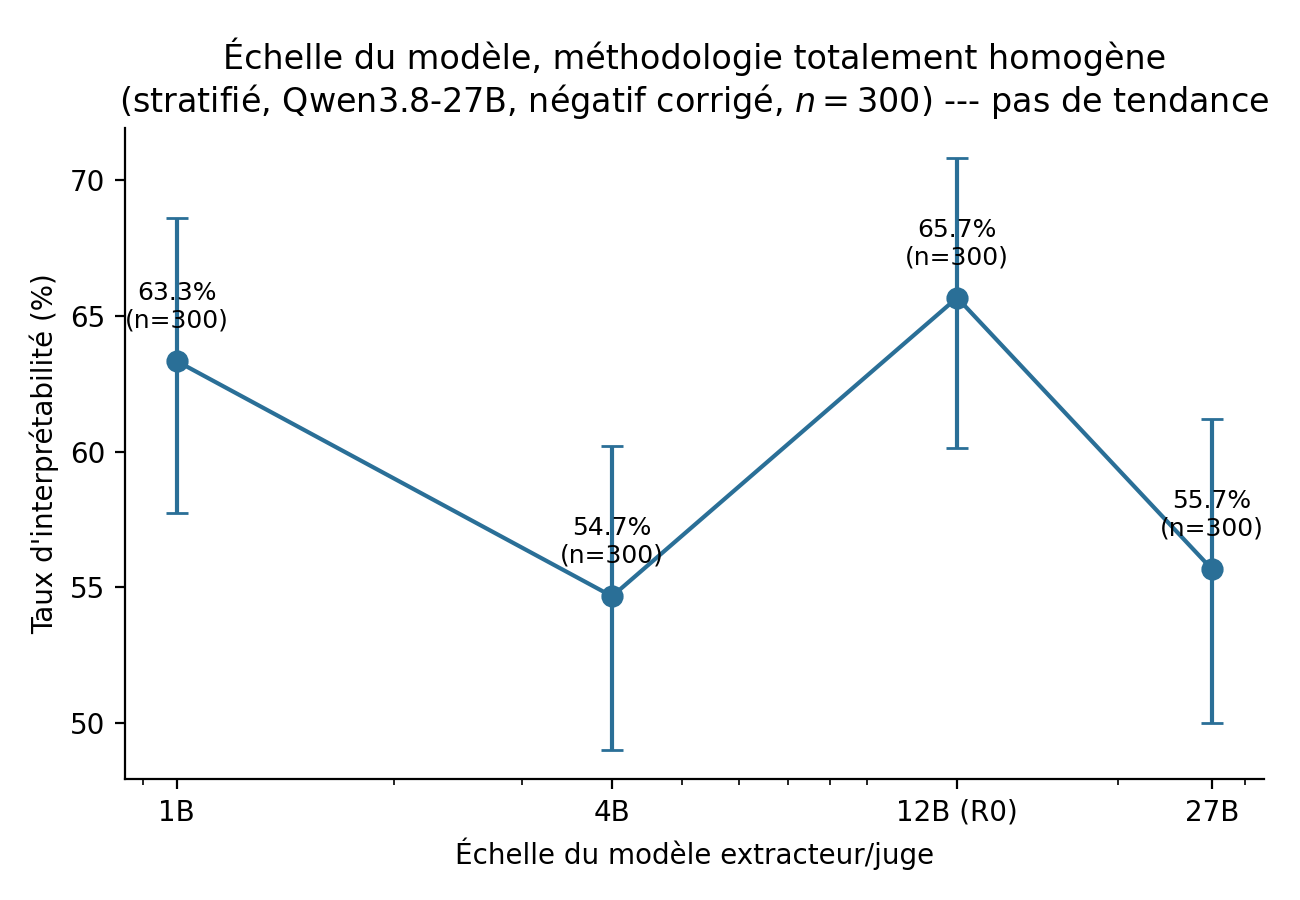
\includegraphics[width=0.75\textwidth]{figures/model_scale_curve.png}}{\fbox{\parbox[c][4cm][c]{0.7\textwidth}{\centering Figure unavailable in standalone review export}}}
\caption{Taux d'interprétabilité par échelle du modèle extracteur/juge,
méthodologie totalement homogène, $n=300$, barres d'erreur = IC95\% de
Wilson. Absence de tendance monotone --- 4B et 27B significativement
\emph{en dessous} de R0 (12B), 1B statistiquement indiscernable de R0.}
\label{fig:model-scale}
\end{figure}

\begin{resultbox}[Effet d'échelle : absence de tendance monotone détectable]
Sous protocole totalement homogène et négatif corrigé, la séquence
1B$\to$4B$\to$12B$\to$27B (63,3\%~$\to$~54,7\%~$\to$~65,7\%~$\to$~55,7\%)
\textbf{n'est pas monotone et ne porte aucune tendance détectable}
(Cochran-Armitage sur les quatre points ordonnés : $z=-0{,}95$,
$p=0{,}34$). Deux paires isolées atteignent la significativité brute contre
R0 (4B : $p=0{,}006$ ; 27B : $p=0{,}012$), mais 1B ne s'en distingue pas
($p=0{,}55$) --- un modèle 12$\times$ plus petit que la référence donne un
taux statistiquement indiscernable de R0, tandis que deux modèles
intermédiaires/plus grands tombent significativement en dessous. \textbf{Ce
n'est pas la signature d'un effet d'échelle} (qui prédirait une progression
ordonnée), \textbf{mais un motif compatible avec du bruit dont R0 est, par
construction, l'un des points hauts} : R0 est la configuration la plus
scrutée et affinée de toute la campagne (\S\ref{subsec:ablations-finales}),
un candidat naturel à être un maximum local de bruit plutôt qu'un véritable
optimum. Cette lecture est corroborée par la correction pour comparaisons
multiples (Benjamini-Hochberg sur l'ensemble des
15 comparaisons contre R0 de ce chapitre) : 4B ($p_\text{BH}=0{,}044$) reste
significatif, mais \textbf{27B ne survit pas à la correction}
($p_\text{BH}=0{,}061$). \textbf{Ces résultats conduisent à reconsidérer
l'hypothèse d'un effet monotone de l'échelle du modèle sur
l'interprétabilité}, telle qu'elle avait été formulée en début de campagne :
les mesures antérieures au correctif de négatif (\S\ref{subsec:audit-negatif})
suggéraient une tendance nette, qui ne survit pas à sa correction.
\end{resultbox}

L'inspection qualitative des hypothèses de diffing générées à chaque échelle
(\emph{cf.}~\S\ref{subsec:diffing}, cohérentes à 12B, confuses à 1B ---
inversion logique cause/conséquence observée) reste, elle, inchangée par ce
qui précède : indépendamment de l'issue chiffrée ci-dessus, la
\textbf{capacité de raisonnement du juge/extracteur} sur des tâches
qualitatives plus exigeantes que l'odd-one-out continue de se dégrader
nettement aux petites échelles.

\subsection{Ablations d'hyperparamètres et de graine sous méthodologie finale}
\label{subsec:ablations-finales}

La campagne d'ablations initiale (14 configurations, Table~\ref{tab:synthese}
en annexe) est intégralement mesurée sous sélection par magnitude et juge
auto-référent --- ses valeurs absolues se lisent comme un plancher, pas comme
le taux réel (\S\ref{subsec:correction-methode}). Le tableau ci-dessous reprend les
hyperparamètres les plus consultés, plus le sweep de \emph{layer}, sous
méthodologie finale (stratifié + Qwen3.8-27B + déduplication + négatif
corrigé, $n=300$), tous comparés à R0 (65,7\%, 197/300) :

\begin{table}[h!]
\centering
\caption{Ablations d'hyperparamètres, de graine et de layer contre R0, méthodologie finale ($n=300$)}
\label{tab:ablations-finales}
\vspace{0.4em}\small
\begin{tabular}{@{}llcccc@{}}
\toprule
\textbf{Run} & \textbf{Écart à R0} & \textbf{Taux interp.} & \textbf{$z$/$p$ vs R0} & \textbf{$p_\text{BH}$} & \textbf{$\Delta$FVE} \\ \midrule
R0 & référence (layer 31) & 65,7\% (197/300) & --- & --- & $+0{,}1393$ \\
V1 & seed 123 (bruit run-à-run) & 63,7\% (191/300) & $z=-0{,}51$, $p=0{,}608$ & $0{,}84$ & $+0{,}1399$ \\
V2 & seed 7 (bruit run-à-run) & 64,0\% (192/300) & $z=-0{,}43$, $p=0{,}669$ & $0{,}84$ & $+0{,}1402$ \\
A1 & $K_\text{extra}=32$ (défaut historique) & \textbf{54,3\% (163/300)} & $z=-2{,}83$, $p=0{,}0046$ & \textbf{0,044} & $+0{,}1483$ \\
A2 & $D_\text{extra}=2048$ (capacité $\times$2) & 67,0\% (201/300) & $z=0{,}35$, $p=0{,}730$ & $0{,}84$ & $+0{,}1468$ \\
A3 & core 65k (défaut : 16k) & 59,0\% (177/300) & $z=-1{,}69$, $p=0{,}092$ & $0{,}28$ & $+0{,}1436$ \\
A4 & $\text{batch}_\text{extra}=16384$ (défaut : 1024) & 65,0\% (195/300) & $z=-0{,}17$, $p=0{,}864$ & $0{,}86$ & $+0{,}1410$ \\
A6 & $\text{épochs}_\text{extra}=40$ (défaut : 10) & 64,7\% (194/300) & $z=-0{,}26$, $p=0{,}797$ & $0{,}85$ & $+0{,}1398$ \\
L1 & layer 24 (défaut historique) & 60,3\% (181/300) & $z=-1{,}35$, $p=0{,}176$ & $0{,}44$ & $+0{,}1163$ \\
L41 & layer 41 & 61,7\% (185/300) & $z=-1{,}02$, $p=0{,}308$ & $0{,}63$ & $+0{,}2200$ \\
layer12 & layer 12 & 74,0\% (222/300) & $z=2{,}22$, $p=0{,}026$ & $0{,}098$ & $+0{,}1574$ \\
\bottomrule
\end{tabular}
\end{table}

\begin{resultbox}[Un seul écart survit à la correction multi-tests : $K_\text{extra}$]
V1 et V2 (deux graines de la configuration de R0, aucun hyperparamètre
changé) donnent \textbf{65,7\% / 63,7\% / 64,0\%} --- un écart de 0,3 point
entre les deux graines, un plancher de bruit run-à-run nettement plus serré
qu'estimé sous l'ancien protocole (8 points) une fois $n$ porté à 300 et le
négatif corrigé. Sur les 15 comparaisons de ce chapitre testées contre R0
(10 ci-dessus, plus les 3 échelles de modèle \S\ref{subsec:model-scale} et
les 2 sanity checks \S\ref{subsec:sanity-check-resultats}), correction
Benjamini-Hochberg appliquée : \textbf{$K_\text{extra}=32$ (A1) est la seule
configuration qui reste significative} ($p_\text{BH}=0{,}044$) --- 54,3\%
contre 65,7\% pour $K_\text{extra}=5$, une chute de plus de 11 points.
Contrairement à la même ablation mesurée à $n=150$ juste après l'adoption du
protocole stratifié+Qwen mais avant le correctif de négatif (A1 non
significatif, 78,0\% contre 84,7\%), \textbf{ce résultat
inverse une conclusion antérieure de ce rapport} : le défaut historique du
dépôt ($K_\text{extra}=32$) est désormais identifié comme la seule ablation
d'hyperparamètre à dégrader mesurablement l'interprétabilité, cohérent avec
le choix de $K_\text{extra}=5$ (optimum du papier SAE Boost) comme
configuration de référence de ce rapport. Le sweep de \emph{layer} ajoute un
signal brut non négligeable (layer12 à 74,0\%, $p=0{,}026$) qui ne survit
cependant pas à la correction ($p_\text{BH}=0{,}098$) --- à confirmer par une
réplication dédiée plutôt qu'à traiter comme acquis.

La colonne $\Delta$FVE (fraction de variance expliquée par le SAE complet,
core+extension, moins celle du core seul --- calculée sur un échantillon de
4096 tokens, indépendante du juge LLM) reste, elle, nettement plus stable sur
le bloc à layer fixe (V1--A6 : $+0{,}1393$ à $+0{,}1483$, écart relatif sous
7\%) mais varie franchement avec le \emph{layer} lui-même (L1 : $+0{,}1163$ ;
L41 : $+0{,}2200$) --- attendu, un point du réseau plus profond laisse
davantage de résidu non expliqué par un cœur GemmaScope entraîné à un point
fixe. Cette dissociation reste cohérente avec le sanity check
\S\ref{subsec:sanity-check-resultats} : le décodeur figé aléatoire y montre
$\Delta$FVE $\approx 0{,}0001$--$0{,}0086$, un facteur ${\sim}16$ à
${\sim}1400$ sous R0, une preuve de falsification nette et indépendante du
bruit de jugement qui domine, lui, le taux d'interprétabilité brut.

Le repère de rigueur retenu pour ce chapitre n'est pas qu'un seuil de
significativité isolé : à $n=300$ par bras et au taux de référence (65,7\%),
le protocole ne détecte qu'un écart d'au moins 10,4 points ($\alpha=0{,}05$,
puissance 80\%) --- une taille d'effet minimale \emph{plus large}, pas plus
étroite, qu'à $n=150$ sous l'ancien taux de référence (9,6 points à
84,7\%), car doubler $n$ ne compense pas le déplacement du taux vers 50\%,
où la variance d'une proportion est maximale. Ce seuil reste cohérent avec
le plancher de bruit empirique mesuré directement entre V1 et V2 (0,3 point)
: le protocole final n'est pas structurellement bruyant, seulement peu
puissant à ce $n$ pour des écarts inférieurs à ${\sim}10$ points --- c'est ce
repère, plus qu'un test isolé, qui borne ce qu'un écart de quelques points
entre deux configurations peut établir dans ce chapitre.
\end{resultbox}

\subsection{Choix des tests et corrections pour comparaisons multiples}
\label{subsec:audit-stats}

Le choix du test statistique a systématiquement suivi la structure de la
comparaison plutôt qu'un test par défaut unique : un test à deux proportions
indépendantes pour deux groupes de features distincts, le test de McNemar
pour les comparaisons appariées sur les mêmes 150 features (biais
multilingue, robustesse du juge, \S\ref{subsec:robustesse}), et le test de
tendance de Cochran-Armitage pour l'effet dose-réponse de l'échelle du
modèle sur un plan à niveaux ordonnés. La correction Benjamini-Hochberg n'a
été appliquée qu'à la campagne finale à $n=300$ de ce chapitre (15
comparaisons contre R0) ; la campagne historique (Table~\ref{tab:synthese},
en annexe), mesurée sous ancien protocole et non corrigée pour comparaisons
multiples, doit être lue en conséquence --- 3 des 14 configurations y
ressortaient significatives sans cette correction (décodeur figé aléatoire,
$z=2{,}86$ ; échelle 4B, $z=3{,}12$ ; échelle 1B, $z=6{,}38$), un chiffre à
ne pas comparer directement au seul écart qui survit à la correction sur le
tableau final ($K_\text{extra}=32$, $p_\text{BH}=0{,}044$).

\medskip
\noindent\textbf{Ce que ce chapitre établit.} Une fois le protocole R0 fixé,
ni l'échelle du modèle testée (1B à 27B) ni la quasi-totalité des
hyperparamètres du SAE ne produisent d'effet robuste à la correction pour
comparaisons multiples ; seul $K_\text{extra}$ s'en distingue. La puissance
disponible à $n=300$ ne permet de détecter que des écarts d'au moins
${\sim}10$ points, un repère à garder à l'esprit pour toute lecture fine de
ce chapitre.

\newpage
% ─────────────────────────────────────────────────────────────────────────────
\section{Résultats : les structures latentes sont-elles stables et identifiables ?}
\label{sec:resultats-stabilite}
% ─────────────────────────────────────────────────────────────────────────────

Une bonne performance globale ne garantit pas que les directions
individuelles du dictionnaire soient elles-mêmes stables ou porteuses d'une
structure sémantique vérifiable. Ce chapitre traite cette question comme un
axe de résultats à part entière, plutôt que comme une simple limite évoquée
en fin de rapport.

\subsection{Stabilité des features et des structures latentes}
\label{subsec:reproductibilite}

La stabilité des features constitue une question distincte de la qualité de leur
interprétation individuelle. Deux expériences complémentaires ont été menées. D'une
part, plusieurs graines d'entraînement donnent des taux globaux très proches sur R0,
mais le recouvrement des labels attribués aux features individuelles entre graines
reste faible (28,2\%). Cela suggère qu'une bonne performance globale ne garantit pas
l'identité des mêmes directions latentes d'un entraînement à l'autre.

D'autre part, le regroupement des features par communautés Louvain a été comparé à un
témoin dans lequel les mêmes objets sont regroupés aléatoirement. Le regroupement
observé n'est pas distinguable du témoin sur le critère utilisé dans cette expérience.
Ce résultat ne signifie pas que le dictionnaire n'apprend aucune structure, mais il
interdit une lecture trop forte du clustering comme preuve, à lui seul, d'une
organisation sémantique stable du latent.

\begin{resultbox}[Ce que les expériences de stabilité permettent d'affirmer]
Les résultats soutiennent une distinction importante entre \textbf{performance globale}
et \textbf{identifiabilité des features individuelles}. Le score d'interprétabilité peut
être stable alors que les coordonnées précises du dictionnaire changent entre graines.
Les regroupements latents doivent donc être considérés comme des objets exploratoires
tant qu'ils ne sont pas séparés d'un témoin aléatoire par un protocole spécifique.
\end{resultbox}

\medskip
\noindent\textbf{Ce que ce chapitre établit.} La performance globale du
protocole d'auto-interprétation est stable entre graines, mais l'identité des
features individuelles ne l'est pas, et le regroupement Louvain n'est pas
distinguable d'un témoin aléatoire sur le critère testé : la structure
latente doit être considérée comme exploratoire tant qu'elle n'est pas
validée par un protocole dédié --- un constat à garder à l'esprit au
chapitre~\ref{sec:resultats-utilite}, où le clustering \emph{ciblé} par
requête donne, lui, un résultat positif.
\newpage
% ─────────────────────────────────────────────────────────────────────────────
\section{Résultats : utilité applicative}
\label{sec:resultats-utilite}
% ─────────────────────────────────────────────────────────────────────────────

Les chapitres précédents portent sur la validité, la fiabilité de mesure et
la stabilité de la représentation elle-même. Ce chapitre évalue sa valeur
pour des tâches avales concrètes, en distinguant explicitement, pour chaque
expérience, ce qui est validé, ce qui est encourageant et ce qui reste
exploratoire.

\subsection{Signal lexical : une baseline indispensable}
\label{subsec:lexical-leakage}

Avant d'interpréter les performances du SAE sur la détection d'intention, il est
nécessaire de vérifier quelle quantité de signal est déjà directement présente dans
le texte. Une expérience de contrôle par TF-IDF montre qu'environ \textbf{93\%} du
signal de classification observé sur les axes étudiés est déjà accessible dans la
représentation lexicale brute. Ce résultat ne discrédite pas le SAE : il fixe une
baseline difficile et empêche surtout d'attribuer au dictionnaire une information
qui provient simplement du vocabulaire.

Cette observation motive directement l'expérience D1 suivante, dans laquelle SAE et
TF-IDF sont évalués sur les mêmes plis et les mêmes labels. Elle permet de séparer une
question d'interprétabilité d'une question d'utilité prédictive.

\subsection{Les codes SAE battent une baseline lexicale honnête sur la détection d'intention}
\label{subsec:d1-intent}

Avant tout résultat d'interprétabilité, une question plus directe : les
codes du dictionnaire SAE sont-ils seulement interprétables, ou aussi
\textbf{utiles} pour une tâche avale concrète ? Cinq intentions client
(réclamation, résiliation, remboursement, demande d'information, urgence),
détectées par mots-clés (\texttt{INTENT\_KEYWORDS\_FR}) sur les 3300 mails
\og{}originaux\fg{} du corpus (pour rappel, un corpus déjà synthétique
antérieur au stage, \emph{cf.}~encadré \S\ref{sec:etat-art} --- pas de la
correspondance client authentique), sont prédites par régression logistique à partir des
codes SAE de R0 et comparées, sur les \textbf{mêmes plis de validation
croisée}, à une baseline TF-IDF+LogReg --- la baseline lexicale la plus
honnête possible face à des labels eux-mêmes construits par mots-clés,
avantage structurel pour TF-IDF a priori. Un test de McNemar apparié par
intention (correction Benjamini-Hochberg sur les 5 tests) évite de conclure
sur un simple écart de moyennes.

\begin{resultbox}[D1 --- SAE contre TF-IDF+LogReg ($n{=}3300$)]
Les codes SAE \textbf{battent ou égalent} TF-IDF+LogReg sur les 5 intentions,
jamais l'inverse : résiliation (98,2\% contre 96,0\%, $p=2{,}9\times10^{-13}$
après BH), remboursement (94,8\% contre 90,4\%, $p=7{,}0\times10^{-22}$) et
information (87,9\% contre 85,6\%, $p=0{,}00084$) significatifs ;
réclamation et urgence à égalité statistique. Contrairement aux résultats
d'interprétabilité des chapitres précédents, ce résultat est mesuré sur
$n=3300$ (pas $n=300$) et n'est pas affecté par le protocole de jugement
odd-one-out (\S\ref{subsec:sanity-check-resultats}) : il ne dépend ni du
juge, ni de la sélection de features, ni de la construction du négatif.
\textbf{Cette expérience apporte un second niveau de validation, indépendant
du protocole d'auto-interprétation, de l'utilité de la représentation SAE
pour une tâche avale concrète.}
\end{resultbox}

\begin{figure}[h!]
\centering
\IfFileExists{figures/d1_intent_bars.png}{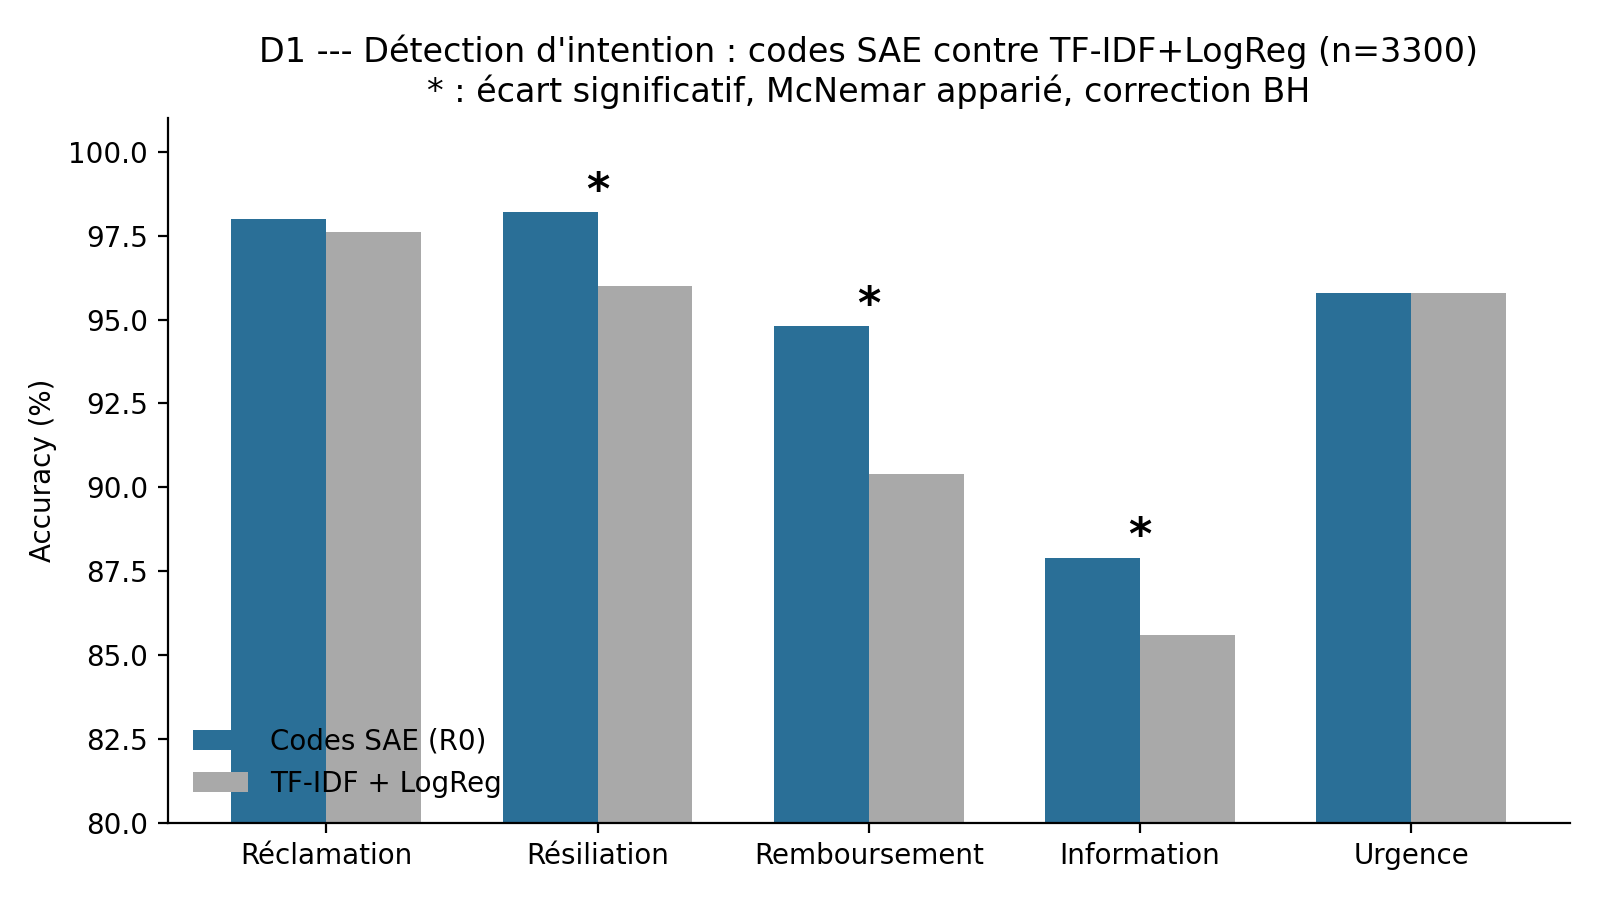
\includegraphics[width=0.85\textwidth]{figures/d1_intent_bars.png}}{\fbox{\parbox[c][4cm][c]{0.8\textwidth}{\centering Figure unavailable in standalone review export}}}
\caption{Accuracy des codes SAE (R0) contre TF-IDF+LogReg sur les 5
intentions client, $n=3300$. Astérisque : écart significatif (McNemar
apparié, correction Benjamini-Hochberg).}
\label{fig:d1-intent}
\end{figure}

\subsection{Qualité de l'explication document-level}

Deux protocoles complémentaires valident que les features citées comme
explication d'une décision de classification y jouent un rôle causal réel,
et non de simples labels plausibles sans lien :

\begin{itemize}
  \item \textbf{Fidélité par ablation} : mettre à zéro les $K$ features les
    plus contributives à une décision de classification produit une chute de
    probabilité prédite nettement supérieure à l'ablation de $K$ features
    aléatoires ou des $K$ moins contributives --- confirmant que les features
    citées comme explication pilotent réellement la décision.
  \item \textbf{Plausibilité par choix forcé} : un juge LLM, confronté aux
    vraies features actives d'un document et à un jeu de features-leurres,
    préfère significativement les vraies features, plus souvent que le
    hasard.
\end{itemize}

\subsection{Retrieval quantitatif (Latent Terms, fusion et reranking)}

\textbf{Latent Terms} \cite{clavie2026latentterms} détourne BM25 --- une
fonction de pertinence classique en recherche d'information, conçue pour
classer des documents à partir de mots-clés --- en remplaçant les mots-clés
par des \textbf{indices de features SAE} : chaque document est représenté par
l'ensemble de ses features actives (son \og{}vocabulaire latent\fg{}), une
requête en langage naturel est elle-même encodée puis réduite à ses features
actives, et BM25 classe les documents par recouvrement de features avec la
requête --- exactement comme il classerait des documents par recouvrement de
mots avec une requête textuelle. Fidèle au protocole du papier, ce SAE est
entraîné par pure reconstruction sur des activations \textbf{token} d'un
corpus générique hors domaine (jamais sur les mails eux-mêmes), puis appliqué
aux mails entiers.

Une évaluation quantitative (Precision@10, 4 intentions en paraphrase, contre
une baseline TF-IDF) ne montre \textbf{pas de victoire uniforme} d'une
méthode : Latent Terms domine largement sur l'intention au taux de base le
plus faible (\emph{remboursement}, 10,3\% : P@10 0,90 contre 0,30 pour
TF-IDF), à égalité sur deux intentions, et dominé par TF-IDF sur l'intention
au taux de base le plus élevé (\emph{réclamation}, 54,8\% : P@10 0,50 contre
1,00 --- TF-IDF profite d'un vocabulaire homogène sur cette intention
précise). Fusionner les deux classements par \textbf{RRF} (\emph{Reciprocal
Rank Fusion}) puis reranker le top-50 avec un juge LLM \textbf{domine
uniformément les 4 intentions} (P@10~$\geq$~0,90 partout, MAP 0,922 contre
0,761 pour RRF seul et 0,678 pour TF-IDF seul) --- premier résultat sans
compromis de cette section. Le \emph{Rank-Biased Overlap} entre les
classements TF-IDF et Latent Terms reste très bas (0,05 en moyenne) même
quand leur précision est proche : les deux méthodes retrouvent des documents
largement différents en tête de liste, ce que le reranking exploite plutôt
que d'arbitrer entre deux versions du même classement.

\subsection{Fidélité du steering (\texttt{steer\_and\_decode})}

Le \textbf{steering} intervient directement sur l'activation d'une feature
(l'amplifier ou la supprimer) pour en observer l'effet causal, plutôt que de
se contenter de la corrélation observationnelle de l'auto-interprétation.
Deux protocoles ont été comparés : l'\textbf{ablation en espace de code}
(effet mesuré directement sur le vecteur latent modifié, sans repasser par
une sortie réelle) et le \textbf{round-trip decode/ré-encode} (le vecteur
modifié est décodé puis ré-encodé, pour vérifier si l'intervention
\emph{survit} au passage par une sortie effectivement utilisable). Le ratio
round-trip/ablation directe quantifie cette survie (proche de 0 : intervention
effacée ; proche de 1 : préservée ; au-delà de 1 : amplifiée).

Jamais testé au-delà d'une vérification géométrique superficielle, ce
protocole révèle, sur les 10 features les plus explicatives de 4 intentions,
un comportement \textbf{très hétérogène selon l'intention} : neutralisé pour
2 intentions sur 4 (ratio 0,00--0,02$\times$), préservé pour une troisième
(0,90$\times$), amplifié pour la dernière (1,74$\times$). Le steering n'est
donc \textbf{pas} un mécanisme d'intervention causale fiable et prévisible en
sortie réelle : une intervention efficace dans l'espace latent peut s'avérer
sans effet une fois le résultat effectivement produit.

\subsection{Diffing entre sous-corpus}
\label{subsec:diffing}

Le \emph{diffing} --- repérer les features dont l'activation diffère entre
deux sous-corpus, pour faire émerger ce qui les distingue --- fait partie des
objectifs initiaux du stage mais n'avait été validé que qualitativement.
Le protocole génère une hypothèse (un concept, à partir des labels de
features dont l'écart de fréquence est marqué entre les deux groupes) puis la
\textbf{vérifie} sur des documents tenus à l'écart de sa génération
(\texttt{verification\_rate}). Faute d'un corpus emails déjà annoté par
sous-catégorie assez large pour ce protocole, la validation porte sur un
sous-corpus générique à deux domaines séparés (énergie \emph{vs.} sport) ---
un banc d'essai pour le \textbf{mécanisme}, avant application au diffing
emails qui a motivé l'objectif initial.

\begin{diagnosticbox}[Résultat exploratoire --- diffing sur corpus proxy ($n{=}10$ hypothèses)]
Une première mesure, à partir des hypothèses les mieux classées par un score
de corrélation archivé, valide 4 hypothèses sur 10
(\texttt{verification\_rate}~=~40,0\%, IC95\% Wilson [16,8\,;\,68,7]\%).
Remplacer cette sélection par une \textbf{génération structurée} (un juge LLM
produit les hypothèses en JSON, avec score de confiance) fait passer le taux
à \textbf{80,0\% (8/10)} --- les 2 hypothèses invalidées sont aussi celles à
la confiance de génération la plus basse (0,75 et 0,65). Le mécanisme de bout
en bout fonctionne sans signe de dégénérescence, et la méthode de génération
des hypothèses affecte le taux de validation au moins autant que la sélection
de features à juger (\S\ref{subsec:correction-methode}). \textbf{Limite} :
$n=10$ hypothèses, un seul tirage de corpus, un corpus générique proxy et non
des emails --- porter cette même chaîne sur un diffing emails reste la suite
naturelle de ce résultat, pas une conclusion à généraliser en l'état.
\end{diagnosticbox}

\subsection{Clustering interprétable de documents}
\label{subsec:clustering}

Le clustering interprétable de documents, second objectif initial resté sans
validation quantitative jusqu'ici, a été exercé de bout en bout sur le
corpus emails : à partir d'une requête en langage naturel (\emph{ex.}
\og{}type de réclamation client\fg{}), un juge LLM génère des mots-clés,
sélectionne les latents de l'extension dont les labels s'y rapportent (union
des \emph{top-k} par mot-clé, 61 features sur les 68 déjà jugées
interprétables), puis regroupe les documents par similarité de Jaccard sur
leur profil d'activation binaire sur ces latents --- une correction de code
a été nécessaire ici, le clustering ciblé utilisant jusque-là une similarité
cosinus sur ce même vecteur binaire, une métrique différente de celle
spécifiée. Chaque cluster obtenu est ensuite étiqueté par un juge LLM, son
accuracy mesurée par réassignation LLM à l'étiquette la plus proche, et sa
\textbf{compacité géométrique} comparée, en espace d'embedding dense
(bge-m3), à des échantillons aléatoires de même taille (\emph{z-conductance} :
négatif si le cluster est plus dense que le hasard) :

\begin{table}[h!]
\centering
\caption{Clustering ciblé sur la requête \og{}type de réclamation client\fg{} (n=300 documents, 4 clusters)}
\label{tab:clustering}
\vspace{0.4em}\small
\begin{tabular}{@{}clcc@{}}
\toprule
\textbf{Cluster} & \textbf{Description (LLM)} & \textbf{Accuracy} & \textbf{$z$-conductance} \\ \midrule
0 (175 doc.) & Résiliation de contrat et litiges de facturation & 61,7\% & $-3{,}12$ \\
1 (25 doc.) & Activation de service et réclamations mixtes & 40,0\% & $-2{,}91$ \\
2 (46 doc.) & Réclamations urgentes pour coupures de courant & 56,5\% & $-4{,}32$ \\
3 (54 doc.) & Demandes administratives mixtes (activation/résiliation) & 5,6\% & $-10{,}06$ \\
\bottomrule
\end{tabular}
\end{table}

Les quatre $z$-conductances sont négatives : les clusters obtenus par
activation SAE sont géométriquement plus compacts, en espace d'embedding
dense, que des échantillons aléatoires de même taille, \textbf{dans le
protocole testé}. Le témoin aléatoire permet de dire que cette compacité est
incompatible avec un tirage aléatoire pour cette requête et ce protocole
précis ; il ne démontre pas, à lui seul, une structure sémantique générale du
dictionnaire --- une lecture plus prudente que celle d'une \og{}preuve de
structure réelle\fg{}, et cohérente avec le témoin Louvain du
chapitre~\ref{sec:resultats-stabilite}, qui ne distingue pas un regroupement
\emph{non ciblé} d'un témoin aléatoire sur un critère différent. L'accuracy
varie en revanche fortement d'un cluster à l'autre (5,6\% à 61,7\%), cohérent
qualitativement avec la littérature citée sur des clusters SAE à variance
d'accuracy plus élevée que des baselines denses : le cluster le moins bien
classé (3) porte lui-même l'étiquette la moins homogène (\og{}demandes
administratives mixtes\fg{}), une correspondance qui a du sens --- compacité
géométrique et cohérence sémantique jugée par LLM ne mesurent pas la même
chose, et peuvent diverger sur un cluster par nature hétérogène.

\textbf{Limite connue des deux résultats ci-dessus} : une seule requête de
clustering testée, aucune baseline dense/instruction-tuned pour situer
l'accuracy en absolu, nombre de clusters fixé sans sélection empirique
(silhouette, \emph{gap statistic}), et --- pour le diffing --- un seul
tirage de corpus par condition ; ces deux protocoles seront réexécutés à
mesure que de nouveaux runs deviennent disponibles.

Ce résultat positif est spécifique au clustering \textbf{ciblé} (guidé par
une requête, restreint aux latents pertinents). Un audit distinct du
clustering \textbf{non ciblé} (HDBSCAN directement sur l'ensemble des codes
SAE documentaires, sans requête) donne un résultat négatif net : sur huit
configurations de réduction de dimension testées (UMAP à différentes
profondeurs, PCA, cosinus brut), la meilleure atteint un score de densité
interne satisfaisant mais aucune ne récupère de structure alignée avec les
14 classes connues du corpus (\emph{Adjusted Mutual Information}
$\approx 0,02$--$0,03$ partout, y compris pour la configuration retenue en
production).

\begin{diagnosticbox}[Résultat exploratoire --- clustering]
Le contraste entre clustering ciblé (compact, guidé par requête) et
clustering non ciblé (AMI $\approx 0$, exploration libre du dictionnaire) est
plus informatif que chacun des deux résultats pris séparément : la structure
latente ne s'auto-organise pas de façon détectable sans une requête qui
restreint l'espace de recherche. Le clustering interprétable de ce dépôt
n'est donc validé que lorsqu'il est guidé par une requête en langage
naturel --- résultat exploratoire (une seule requête testée pour le
clustering ciblé), à confirmer sur un plus grand nombre de requêtes avant
généralisation.
\end{diagnosticbox}

\subsection{Pipeline 2 : backbone d'embedding et interprétabilité}
\label{subsec:pipeline2-scale}

Un balayage de quatre backbones d'embedding (F2LLM-v2 80M/160M/330M, bge-m3)
et de la dimension MRL de F2LLM est détaillé en annexe~\S\ref{app:pipeline2}
: bge-m3 domine nettement les métriques de reconstruction (NMSE $-18,8\%$,
4 à 5$\times$ moins de features mortes) sans avoir été adopté comme défaut de
production, faute de comparaison chiffrée sur l'interprétabilité elle-même ;
la dimension d'embedding se dégrade graduellement, pas abruptement (10\% des
dimensions conservent 94\% de la performance de classification).

Sur l'\textbf{interprétabilité} du Pipeline~2 lui-même, mesurée sous le même
protocole que Pipeline~1 (sélection stratifiée, juge Qwen3.8-27B), le taux
atteint \textbf{58,7\% (88/150)} --- proche de la référence Pipeline~1
(65,7\%), alors que sa reconstruction est bonne et non dégradée. Ce chiffre
utilise une construction du négatif structurellement différente de
Pipeline~1 (la phrase candidate entière est affichée, sans fenêtre de
contexte centrée sur un argmax) : vérifié directement, négatifs et positifs
y ont des longueurs statistiquement indissociables (16,8 contre 15,6 mots en
moyenne, contre un facteur ${\sim}23\times$ pour Pipeline~1 avant correctif),
et la longueur du négatif ne prédit pas le succès du juge (Spearman
$\rho=0,069$, $p=0,40$) --- le biais décrit en \S\ref{subsec:audit-negatif}
ne s'y réplique pas, 58,7\% n'a pas besoin d'être requalifié pour ce motif.
Pipeline~2 fonctionne de bout en bout et reconstruit bien, mais son
interprétabilité individuelle reste, à ce stade, inférieure à Pipeline~1.

\medskip
\noindent\textbf{Ce que ce chapitre établit.} Indépendamment du score
d'auto-interprétation, les codes SAE égalent ou battent une baseline
lexicale honnête sur cinq tâches d'intention réelles, produisent des
explications causalement fidèles, et permettent un retrieval et un
clustering guidés par requête utiles --- sans qu'un signal équivalent
émerge d'une exploration non guidée du dictionnaire (diffing sur corpus
proxy, clustering non ciblé, steering hétérogène). Les résultats de ce
chapitre marqués \og{}résultat exploratoire\fg{} appellent une réplication
avant généralisation ; les autres (D1, fidélité de l'explication, retrieval
avec reranking) sont mesurés à une échelle ($n\geq 300$) qui en fait des
résultats robustes indépendamment du protocole de jugement odd-one-out.
\newpage
% ─────────────────────────────────────────────────────────────────────────────

\section{Discussion et conclusion}
\label{sec:discussion}
% ─────────────────────────────────────────────────────────────────────────────

\subsection{Bilan par rapport aux objectifs initiaux}

\begin{table}[h!]
\centering
\caption{Bilan par rapport aux étapes de l'offre de stage}
\vspace{0.4em}\small
\begin{tabular}{@{}p{5.5cm}p{8.5cm}@{}}
\toprule
\textbf{Étape prévue} & \textbf{Réalisation} \\ \midrule
Partie bibliographique sur les SAE & Faite --- élargie à un panorama des
  architectures, des embeddings, des lois d'échelle, et de la littérature de
  sanity-check récente (chapitre~\ref{sec:etat-art}). \\
Choix d'une implémentation existante & GemmaScope + SAELens comme cœur
  préentraîné, complété d'une extension développée pendant le stage. \\
Conversion des données en embeddings & Deux pipelines indépendants
  (Gemma-3/GemmaScope, F2LLM/bge-m3). \\
Entraînement d'un SAE & Fait, avec diagnostic et correction d'un défaut de
  corpus majeur en cours de route. \\
Analyses, interprétation, visualisation & Dashboard interactif, juge LLM
  automatisé, retrieval, diffing, clustering interprétable, sondes de
  classification. \\
Rédaction d'un rapport & Ce document. \\
\bottomrule
\end{tabular}
\end{table}

\subsection{Ce qui est établi}

Quatre constats reposent sur des métriques indépendantes du juge LLM ou sur
des tailles d'échantillon suffisantes pour être considérés comme robustes
dans le cadre de ce stage :
\begin{itemize}
  \item l'extension à cœur gelé apprend une information résiduelle réelle,
  au sens du $\Delta$FVE et du $\Delta$CE (chapitre~\ref{sec:resultats-representation}) ;
  \item le protocole de mesure de l'interprétabilité (sélection des
  features, juge, construction du négatif) domine tout effet d'architecture
  ou d'échelle testé dans ce rapport (chapitre~\ref{sec:resultats-mesure}) ;
  \item l'effet d'échelle du modèle, formulé en début de campagne comme une
  hypothèse de travail centrale, ne se réplique pas sous protocole corrigé
  et correction pour comparaisons multiples (chapitre~\ref{sec:resultats-robustesse}) ;
  \item les codes SAE sont utiles pour la détection d'intention sur les
  mails du corpus, à performance égale ou supérieure à une baseline
  lexicale honnête, indépendamment du juge (chapitre~\ref{sec:resultats-utilite}).
\end{itemize}

\subsection{Ce qui ne l'est pas}

D'autres résultats restent ouverts ou insuffisamment répliqués, et ne
doivent pas être lus comme des conclusions établies :
\begin{itemize}
  \item l'identité des features individuelles entre graines d'entraînement
  (28,2\% de recouvrement) et la structure de regroupement Louvain (non
  distinguable d'un témoin aléatoire) --- chapitre~\ref{sec:resultats-stabilite} ;
  \item le signal isolé du layer 12 ($p=0{,}026$, non significatif après
  correction Benjamini-Hochberg), qui appelle une réplication dédiée plutôt
  qu'une généralisation ;
  \item le diffing et le clustering ciblé, validés respectivement sur un
  corpus proxy générique et sur une seule requête --- résultats
  exploratoires et non des validations définitives (chapitre~\ref{sec:resultats-utilite}) ;
  \item l'extrapolation au-delà de 25M tokens, la borne à 200M n'ayant
  jamais été menée à terme.
\end{itemize}

\subsection{Apports et résultats principaux}

Les résultats du stage peuvent être regroupés en quatre contributions complémentaires,
plutôt qu'en une seule découverte dominante.

\begin{enumerate}
  \item \textbf{Validation de l'architecture à cœur gelé.} Le $\Delta$FVE et le
  $\Delta$CE fournissent deux validations indépendantes du juge LLM : l'extension
  apprend une information résiduelle substantielle et causalement utile, tandis que
  les décodeurs figés aléatoires ne reproduisent pas cette capacité.

  \item \textbf{Caractérisation du protocole d'auto-interprétation.} La sélection par
  magnitude et la sélection stratifiée sondent des populations de features différentes,
  et le choix du juge ainsi que la construction du négatif peuvent déplacer fortement
  le taux observé. Le protocole final résulte donc d'une campagne d'audit et non d'un
  choix arbitraire de paramètres.

  \item \textbf{Réévaluation de l'effet d'échelle et des hyperparamètres.} Une fois le
  protocole stabilisé, l'échelle 1B--27B ne présente pas de tendance monotone détectable.
  Parmi les ablations finales, seul $K_\text{extra}=32$ reste significativement différent
  de R0 après correction Benjamini--Hochberg. Le stage ne permet donc pas de conclure
  que l'augmentation de l'échelle du modèle améliore l'interprétabilité dans les
  conditions étudiées.

  \item \textbf{Limites de la stabilité et utilité avale.} Les features individuelles
  ne sont pas parfaitement reproductibles entre graines et certains regroupements ne
  se distinguent pas d'un témoin aléatoire. En parallèle, les codes SAE restent
  compétitifs avec TF-IDF sur cinq tâches de détection d'intention, ce qui fournit une
  validation applicative indépendante de l'odd-one-out.
\end{enumerate}

Ces quatre axes forment une chaîne de validation : apprendre une représentation utile,
mesurer correctement son interprétabilité, tester la robustesse des conclusions, puis
évaluer une utilité indépendante du score d'explication. Cette organisation, reprise
par la structure même de ce rapport (chapitres~\ref{sec:resultats-representation} à
\ref{sec:resultats-utilite}), est plus informative qu'une lecture chronologique des
nombreuses ablations réalisées au cours du stage.

\subsection{Points non résolus et perspectives}

\textbf{Pistes délibérément abandonnées.} Au vu de l'ampleur de la campagne
de correction méthodologique menée sur le protocole de mesure lui-même
(\S\ref{subsec:correction-methode}, \S\ref{subsec:sanity-check-resultats}),
plusieurs directions envisagées en phase bibliographique ou préliminaire ont
été dépriorisées plutôt que menées à mi-chemin : l'architecture Matryoshka
pleinement hiérarchique (dictionnaires emboîtés à plusieurs niveaux ---
l'architecture à cœur gelé testée n'a qu'un seul niveau d'extension) ; un
pipeline micro/macro à deux SAE alignés par \emph{AlignedUMAP} (projection 2D
contraignant les positions à rester comparables d'un sous-corpus à l'autre) ;
une modélisation par graphe biparti (documents et features comme deux
ensembles de nœuds reliés par les activations, pour en exploiter la structure
de communautés) ; et un protocole d'annotation humaine avec calcul du
$\kappa$ de Fleiss pour remplacer le juge LLM par une validation humaine d'un
sous-échantillon. Aucune comparaison chiffrée directe n'a non plus été menée
contre les baselines alternatives de SAE Boost (Extended SAE à
initialisation aléatoire/most-active, SAE Stitching, fine-tuning complet).

\textbf{Écarts réels à combler.} Le découplage juge/extracteur
(\S\ref{subsec:correction-methode}) ne fait varier que le juge, à extracteur
fixe (Gemma-3-12B-it) : isoler pleinement la capacité d'\emph{extraction} de
celle du \emph{jugement} demanderait un plan croisé complet --- modèle léger
comme extracteur et comme juge, modèle léger comme extracteur mais juge
capable, et l'inverse --- non mené ici. Le balayage d'échelle
(\S\ref{subsec:model-scale}) montre par ailleurs un motif non monotone
(1B$\approx$R0 > 4B$\approx$27B) qui reste, en l'état, sans explication
mécanique : une réplication sur une seconde graine à chaque échelle
permettrait de trancher si ce motif est stable ou un artefact de bruit sur
un seul tirage par point. En raison d'une contrainte d'indexation apparue
lors d'une évolution antérieure du format du corpus augmenté, l'appariement
entre chaque mail original et ses variantes repose actuellement sur un
alignement positionnel plutôt que sur l'identification prévue par empreinte
de contenu --- fragile en principe (une modification ultérieure du corpus
source désynchroniserait silencieusement cet appariement), mais sans
conséquence à ce jour puisque ce corpus source n'a pas changé depuis la
génération des variantes. Corriger cet alignement à la source reste possible
mais impliquerait de régénérer l'ensemble du corpus augmenté et, avec lui,
le cache d'extraction partagé de toute la campagne --- un chantier hors de
portée avant la soutenance au vu du gain attendu.
Le diffing (\S\ref{subsec:diffing}) n'a par ailleurs été validé que sur un
sous-corpus générique proxy (énergie \emph{vs.} sport) --- porter la même
chaîne (génération d'hypothèses structurée, vérification sur documents tenus
à l'écart) sur un diffing emails (\emph{ex.} urgents \emph{vs.} non urgents),
l'objectif initial qui a motivé cette fonctionnalité, reste à faire. Une
tentative d'ablation de volume à 200M tokens (borne haute exacte du seuil de
convergence revendiqué par SAE Boost, contre 25M dans la configuration de
référence) a été lancée mais n'a jamais abouti (job annulé lors d'un
incident cluster) et n'a pas été relancée --- l'absence d'effet mesurable du
volume jusqu'à 25M (Table~\ref{tab:synthese}) reste donc non extrapolée
au-delà de cette borne.

\textbf{Contraintes d'écosystème.} CamemBERTav2 et Qwen3-Embedding,
identifiés en phase bibliographique comme candidats sérieux pour le
Pipeline~2, n'ont pas été intégrés faute d'écosystème SAE préentraîné
équivalent à GemmaScope --- une comparaison chiffrée directe reste à faire
si l'équipe souhaite objectiver ce choix par rapport au score MTEB plutôt
que par la seule disponibilité d'infrastructure.

\textbf{Apports pour EDF.} Au-delà des résultats méthodologiques, ce stage
laisse une chaîne d'analyse directement réutilisable pour la correspondance
client : un pipeline d'extraction de features interprétables sur mails
français, un protocole d'évaluation audité (dont les biais identifiés
--- sélection, juge, négatif --- sont transférables à tout futur projet
d'auto-interprétation par juge LLM chez EDF), et une validation applicative
concrète sur cinq intentions client (chapitre~\ref{sec:resultats-utilite}),
compétitive avec une baseline lexicale déjà en place. Le retrieval par
fusion RRF~+~reranking constitue le résultat le plus directement
opérationnalisable du stage pour une recherche de mails par propriété.

\subsection{Conclusion générale}

Ce stage a conduit à la construction et à l'évaluation d'une chaîne complète pour
l'analyse interprétable de représentations textuelles par Sparse Autoencoders, avec
un cas d'usage orienté vers la correspondance client d'EDF. Le travail ne se résume
pas à l'obtention d'un taux d'interprétabilité élevé : l'enjeu a progressivement été
de déterminer quelles propriétés de la représentation et quelles propriétés du
protocole expérimental pouvaient réellement être établies.

Le premier résultat solide est architectural. L'extension à cœur gelé apprend une
quantité mesurable d'information résiduelle : sous R0, $\Delta$FVE vaut $+0{,}1393$,
contre seulement $+0{,}0001$ à $+0{,}0086$ pour les témoins à décodeur aléatoire. Une
mesure indépendante fondée sur la cross-entropy confirme cette différence causale.
Ces résultats ne dépendent ni du juge LLM ni du document négatif du protocole
\emph{odd-one-out}.

Le deuxième résultat concerne la mesure elle-même. La comparaison entre sélection par
magnitude et sélection stratifiée montre que la population de features évaluée est
une variable scientifique à part entière. À cela s'ajoutent l'indépendance du juge et
la construction du négatif. L'audit de cette chaîne a conduit à retenir 65,7\% comme
estimation de référence sous protocole corrigé, plutôt que les taux historiques plus
élevés obtenus avec des conditions biaisées. Cette conclusion ne signifie pas que le
protocole précédent était inutile : il a permis de révéler que le score devait être
traité comme une mesure expérimentale à auditer, et non comme une propriété intrinsèque
observée directement.

Le troisième résultat est une réévaluation de l'hypothèse d'échelle. L'expérience
1B--4B--12B--27B ne montre aucune tendance monotone détectable après correction des
biais du protocole et des comparaisons multiples. L'hypothèse initiale d'un effet
croissant avec la taille du modèle n'est donc pas soutenue dans les conditions testées.
Le seul hyperparamètre SAE qui survit à la campagne finale est $K_\text{extra}$, dont
la valeur historique 32 dégrade le taux d'interprétabilité de plus de 11 points par
rapport à R0.

Enfin, les expériences de stabilité et d'application montrent les limites et les
possibilités de la représentation. Le faible recouvrement des features individuelles
entre graines et le témoin de regroupement aléatoire invitent à ne pas confondre
interprétabilité locale et identifiabilité globale. À l'inverse, la comparaison avec
TF-IDF sur 3300 mails montre que les codes SAE peuvent être au moins aussi performants
qu'une baseline lexicale sur cinq tâches d'intention, indépendamment du juge LLM.

Le résultat général du stage est ainsi méthodologique : une représentation SAE ne peut
être considérée comme interprétable sur la seule base d'un score d'auto-évaluation.
Il faut distinguer au minimum la qualité de reconstruction, la fidélité causale,
la procédure d'échantillonnage, la robustesse du jugement, la stabilité des features
et l'utilité sur une tâche avale. Cette chaîne fournit un cadre de validation plus
robuste pour la poursuite du travail chez EDF, tout en laissant ouvertes plusieurs
questions : réplication inter-seed de l'étude d'échelle, validation du diffing sur des
emails réellement annotés par sous-catégorie, comparaison de backbones supplémentaires
et étude plus systématique de l'identifiabilité des sous-espaces latents.

\appendix
\section{Traçabilité des premières ablations}

La première campagne de 14 ablations a été réalisée sous sélection par magnitude et
juge auto-référent. Elle est conservée ici pour la traçabilité du projet, mais ses
valeurs absolues ne constituent pas les estimations finales de l'interprétabilité.
Les comparaisons internes restent utiles pour comprendre quelles variables ont été
retenues pour la campagne finale.

\begin{table}[!ht]
\centering
\caption{Campagne initiale de 14 ablations --- sélection par magnitude, juge
auto-référent, négatif non corrigé (à lire comme plancher relatif, pas comme
taux réel ; \emph{cf.}~\S\ref{subsec:model-scale} et \S\ref{subsec:ablations-finales}
pour les valeurs correspondantes sous protocole final)}
\label{tab:synthese}
\small
\begin{tabular}{@{}lcc@{}}
\toprule
Configuration & Taux historique & Statut dans l'analyse finale \\
\midrule
Volume 100k tokens & 40,7\% & non significatif \\
Volume 2M tokens & 44,7\% & non significatif \\
Volume 25M tokens & 54,0\% & non significatif \\
Largeur core 65k & 43,3\% & vérifiée sous protocole final \\
Largeur core 262k & 46,7\% & vérifiée sous protocole final \\
Époques $\times4$ & 41,3\% & vérifiée sous protocole final \\
Capacité combinée & 40,0\% & vérifiée sous protocole final \\
$D_\text{extra}=2048$ & 46,0\% & vérifiée sous protocole final \\
$K_\text{extra}=5$ & 54,7\% & configuration retenue \\
Seed 123 & 47,3\% & réplication finale \\
Décodeur aléatoire & 29,3\% & sanity check requalifié \\
Échelle 4B & 28,0\% & effet non répliqué \\
Échelle 1B & 12,0\% & effet non répliqué \\
Combiné v12 & 44,0\% & exploratoire \\
\bottomrule
\end{tabular}
\end{table}

\section{Détail du choix de backbone d'embedding (Pipeline 2)}
\label{app:pipeline2}

\begin{table}[!ht]
\centering
\caption{Comparaison des backbones d'embedding du Pipeline~2 (reconstruction
uniquement --- interprétabilité mesurée séparément, \S\ref{subsec:pipeline2-scale})}
\small
\begin{tabular}{@{}lcccc@{}}
\toprule
Métrique & F2LLM-80M & F2LLM-160M & F2LLM-330M & bge-m3 \\ \midrule
NMSE & 0,0745 & 0,0727 & 0,0689 & \textbf{0,0559} \\
dead\% & 0,63\% & 0,77\% & 0,70\% & \textbf{0,13\%} \\
$\rho_\text{SAE}$ & 0,9597 & 0,9531 & 0,9574 & 0,9303 \\
silhouette & 0,0212 & 0,0193 & 0,0183 & \textbf{0,0228} \\
acc\_SAE (diffing) & 0,665-0,672 & 0,670 & 0,687 & \textbf{0,697} \\
\bottomrule
\end{tabular}
\end{table}

Balayage de la dimension d'embedding \texttt{MATRYOSHKA\_DIM} (F2LLM-160M,
dimensions 64/128/320/640) : pour F2LLM-80M, la dimension par défaut égale
exactement la dimension complète du modèle, rendant toute troncature
antérieure un artefact sans effet réel sur ce backbone --- jamais remarqué
avant cette vérification. Sur F2LLM-160M, la classification aval se dégrade
de façon graduelle avec la troncature (72,8\% à 64 dimensions contre 77,4\%
au complet), \textbf{10\% des dimensions conservant déjà 94\% de la
performance du plein embedding} --- cohérent avec, sans le démontrer
formellement, un comportement de type Matryoshka.

\section{Résultats exploratoires et pistes abandonnées}

Les résultats de diffing (\S\ref{subsec:diffing}) et de clustering ciblé
(\S\ref{subsec:clustering}) sont présentés dans le corps du rapport,
signalés chacun par un encadré \og{}résultat exploratoire\fg{} dédié plutôt
que renvoyés en annexe : ils restent des pistes utiles, pas des validations
définitives. Le balayage MRL (annexe~\ref{app:pipeline2}) et le run à 200M
tokens (jamais abouti, \emph{cf.}~\S\ref{sec:discussion}) complètent ces
pistes sans validation supplémentaire à ce stade. Les limitations détaillées
au chapitre Discussion précisent les conditions nécessaires à leur
consolidation.

\newpage
% =============================================================================
% BIBLIOGRAPHIE
% =============================================================================
\addcontentsline{toc}{section}{Bibliographie}
\begin{thebibliography}{99}\small

\bibitem{elhage2022superposition}
  Elhage, N. et al.
  \textit{Toy Models of Superposition}.
  Transformer Circuits Thread, Anthropic, 2022.

\bibitem{bricken2023monosemanticity}
  Bricken, T. et al.
  \textit{Towards Monosemanticity: Decomposing Language Models With Dictionary Learning}.
  Transformer Circuits Thread, Anthropic, 2023.

\bibitem{cunningham2023sparse}
  Cunningham, H., Ewart, A., Riggs, L., Huben, R., \& Sharkey, L.
  \textit{Sparse Autoencoders Find Highly Interpretable Features in Language Models}.
  ICLR 2024. arXiv:2309.08600.

\bibitem{rajamanoharan2024gated}
  Rajamanoharan, S. et al.
  \textit{Improving Dictionary Learning with Gated Sparse Autoencoders}.
  arXiv:2404.16014, 2024.

\bibitem{gao2024topk}
  Gao, L. et al.
  \textit{Scaling and Evaluating Sparse Autoencoders}.
  arXiv:2406.04093, OpenAI, 2024.

\bibitem{bussmann2025batchtopk}
  Bussmann, B., Nabeshima, N., Karvonen, A., \& Nanda, N.
  \textit{Learning Multi-Level Features with Matryoshka Sparse Autoencoders}.
  ICML 2025. arXiv:2503.17547.

\bibitem{rajamanoharan2024jumprelu}
  Rajamanoharan, S. et al.
  \textit{Jumping Ahead: Improving Reconstruction Fidelity with JumpReLU Sparse Autoencoders}.
  arXiv:2407.14435, DeepMind, 2024.

\bibitem{bussmann2025matryoshka}
  Bussmann, B., Nabeshima, N., Karvonen, A., \& Nanda, N.
  \textit{Learning Multi-Level Features with Matryoshka Sparse Autoencoders}.
  ICML 2025. arXiv:2503.17547.

\bibitem{templeton2024scaling}
  Templeton, A. et al.
  \textit{Scaling Monosemanticity: Extracting Interpretable Features from Claude 3 Sonnet}.
  Anthropic, 2024.

\bibitem{bloom2024saelens}
  Bloom, J., Tigges, C., Duong, A., \& Chanin, D.
  \textit{SAELens}. \url{https://github.com/decoderesearch/SAELens}, 2024.

\bibitem{jiang2024sae_embeddings}
  (Collectif MATS).
  \textit{Interpretable Embeddings with Sparse Autoencoders: A Data Analysis Toolkit}.
  arXiv:2512.10092, 2024.

\bibitem{decodedense2025}
  (Anonyme).
  \textit{Decoding Dense Embeddings: Sparse Autoencoders for Interpreting and Discretizing Dense Retrieval}.
  arXiv:2506.00041, 2025.

\bibitem{kusupati2022mrl}
  Kusupati, A. et al.
  \textit{Matryoshka Representation Learning}.
  NeurIPS 2022.

\bibitem{koriagin2025saeboost}
  Koriagin, N., Aksenov, Y., Laptev, D., Gerasimov, G., Balagansky, N., \& Gavrilov, D.
  \textit{Teach Old SAEs New Domain Tricks with Boosting}.
  arXiv:2507.12990, 2025.

\bibitem{korznikov2025sanitychecks}
  Korznikov, A., Galichin, A., Dontsov, A., Rogov, O., Oseledets, I., \& Tutubalina, E.
  \textit{Sanity Checks for Sparse Autoencoders: Do SAEs Beat Random Baselines?}
  arXiv:2602.14111, 2025.

\bibitem{lieberum2024gemmascope}
  Lieberum, T. et al.
  \textit{Gemma Scope: Open Sparse Autoencoders Everywhere All At Once on Gemma 2}.
  arXiv:2408.05147, Google DeepMind, 2024.

\bibitem{resck2025multilingual}
  Resck, L., Augenstein, I., \& Korhonen, A.
  \textit{Explainability and Interpretability of Multilingual LLMs: A Survey}.
  EMNLP 2025.

\bibitem{clavie2026latentterms}
  Clavié, B., Lee, S., Shakir, A., Kato, M. P.
  \textit{Latent Terms: Dense Retrievers Contain Trivially Extractable BM25-ready Zipfian Vocabularies}.
  arXiv:2605.29384, 2026.

\bibitem{unstablefeatures2026}
  (Anonyme).
  \textit{Unstable Features, Reproducible Subspaces}.
  arXiv:2606.12138, 2026.

\bibitem{identifiablesae2026}
  (Anonyme).
  \textit{Toward Identifiable Sparse Autoencoders}.
  arXiv:2605.31245, 2026.

\bibitem{multilingualconcepts2025}
  (Anonyme).
  \textit{Sparse Autoencoders Can Capture Language-Specific Concepts Across Diverse Languages}.
  arXiv:2507.11230, 2025.

\bibitem{beckmannqueloz2026}
  Beckmann, P. \& Queloz, M.
  \textit{Mechanistic Indicators of Understanding in Large Language Models}.
  2026.

\bibitem{bills2023language}
  Bills, S. et al.
  \textit{Language Models Can Explain Neurons in Language Models}.
  OpenAI, 2023.

\bibitem{karvonen2025saebench}
  Karvonen, A. et al.
  \textit{SAEBench: A Comprehensive Benchmark for Sparse Autoencoders in
  Language Model Interpretability}.
  arXiv:2503.09532, ICML 2025.

\bibitem{formal2026splare}
  Formal, T., Louis, M., Déjean, H., \& Clinchant, S.
  \textit{Learning Retrieval Models with Sparse Autoencoders}.
  arXiv:2603.13277, NAVER LABS Europe, 2026.

\end{thebibliography}

\end{document}
